\documentclass{VUMIFPSbakalaurinis}
\usepackage{algorithmicx}
\usepackage{algorithm}
\usepackage{algpseudocode}
\usepackage{amsfonts}
\usepackage{amsmath}
\usepackage{bm}
\usepackage{caption}
\usepackage{color}
\usepackage{float}
\usepackage{graphicx}
\usepackage{listings}
\usepackage{subfig}
\usepackage{wrapfig}
\usepackage{makecell}
\usepackage{multirow}
\usepackage{forest}
\usepackage{pgfplots}

\usepackage{enumitem}
\setlist{noitemsep, topsep=0pt}

\renewcommand\theadfont{\bfseries}
\newcommand\tab[1][1cm]{\hspace*{#1}}


\definecolor{myyellow}{RGB}{154, 125, 10}
\definecolor{myred}{RGB}{199, 0, 57}
\definecolor{myblue}{RGB}{52, 152, 219}
\definecolor{mygreen}{RGB}{30, 132, 73}


% Titulinio aprašas
\university{Vilniaus universitetas}
\faculty{Matematikos ir informatikos institutas}
\department{Programų sistemų katedra}
\papertype{Bakalauro darbas}
\title{Gestų kalbos vienetų atpažinimas iš video srauto}
\titleineng{Recognition of Sign language units from a video stream}
\author{Pranciškus Ambrazas}
\supervisor{j. asist. Linas Petkevičius}
\reviewer{dr. Vytautas Valaitis}
\date{Vilnius – \the\year}

% Nustatymai
% \setmainfont{Palemonas}   % Pakeisti teksto šriftą į Palemonas (turi būti įdiegtas sistemoje)
\bibliography{bibliografija}

\begin{document}
\maketitle

%% Padėkų skyrius
% \sectionnonumnocontent{}
% \vspace{7cm}
% \begin{center}
%     Padėkos asmenims ir/ar organizacijoms
% \end{center}

\sectionnonumnocontent{Santrauka}

Šiame darbe nagrinėjamas lietuvių gestų kalbos atpažinimas iš video srauto. Buvo susikurta lietuvių gestų kalbos duomenų bazė, kurią sudaro 22 gestai po 20 vaizdo įrašų kiekvienai klasei ir 3 gestai po 50 vaizdo įrašų kiekvienai klasei. Klasių, kurios turėjo po 20 vaizdo įrašų, video srautai buvo transformuojami, kad kiekviena klasė turėtų po 50 vaizdinių įrašų. Remiantis šiais duomenimis buvo apmokomas konvoliucinis neuroninis tinklas pasinaudojant \textit{Inception v3} modeliu. Toliau, remiantis konvoliucinio neuroninio tinklo rezultatais, buvo apmokomas rekurentinis neuroninis tinklas. Galiausiai buvo sukurti trys skirtingi modeliai, gebantys atitinkamai atpažinti 3, 10 ir 25 skirtingas lietuvių gestų kalbos klases. Geriausius rezultatus davė 10 klasių modelis (87,34\%), tačiau didesnį panaudojamumą turi 25 lietuvių gestų kalbos klasių modelis, kuris 79,18\% tikslumu atspėja rodomo gesto klasę. Taigi galima daryti išvadą, kad gauti rezultatai duoda pakankamą tikslumą norint šį modelį pritaikyti realiame pasaulyje. Apmokius jį atpažinti daugiau klasių, panaudojamumas taptų žymiai didesnis.

% Nurodomi iki 5 svarbiausių temos raktinių žodžių (terminų).
% Vienas terminas gali susidėti iš kelių žodžių.
\raktiniaizodziai{konvoliuciniai neuroniniai tinklai, rekurentiniai neuroniniai tinklai, lietuvių gestų kalba, apsimokančios sistemos}   

\sectionnonumnocontent{Summary}

In this study the recognition of Sign language units from a video stream is being analyzed. A dataset of 22 sign units with 20 videos for each class and 3 units with 50 videos for each class was created. Classes which had 20 videos was augmented to make 50 videos for each one of them. Based on this data, the convolutional neural network using Inception v3 model was trained. Further, based on convolutional neural network results, recurrent neural network was trained. Finally, three different models was created which are able to detect 3, 10 and 25 Lithuanian Sign language classes. The best results was presented by 10 classes model (87,34\%), but 25 signs model has a higher usability within 79,18\% accuracy. To sum up, these results give a possibility to adapt Lithuanian Sign language models in a real world. The usability of this model can be increased by further studies and trainings.

\keywords{convolutional neural networks, recurrent neural networks, lithuanian sign language, machine learning}

\tableofcontents

\sectionnonum{Įvadas}
Pasaulyje yra virš 7 milijardų žmonių, kurie kasdien tarpusavyje komunikuoja. Net 5\% visos žmonijos populiacijos sudaro žmonės, turintys klausos problemų, dėl kurių jiems sunkiau komunikuoti tarpusavyje. Vien 34 milijonai iš jų yra vaikai, iš kurių net 60\% praradusių klausą vaikystėje galėjo būti girdintys dabar, jei būtų imtąsi atitinkamų prevencinių priemonių. Paskaičiuota, kad iki 2050 metų žmonių, turinčių šias problemas, skaičius išaugs netgi iki 900 milijonų. Vien šiuo metu 1,1 milijardo jaunų žmonių nuo 11 iki 35 metų amžiaus yra ant klausos praradimo ribos dėl per didelio triukšmo \cite{WhoInt}.

\subsectionnonum{Gestų kalba}
Gestų kalba – tai geriausias būdas klausos negalią turintiems žmonėms bendrauti tarpusavyje. Ja pasaulyje bendrauja didžioji dalis klausos sutrikimus turinčiųjų, o amerikiečių gestų kalba (\textit{angl. American Sign Language (toliau - ASL)}) yra trečia pagal populiarumą Amerikoje ne anglų kalba po ispanų ir kinų kalbų ir ketvirta apskirtai, kuria kalba virš 500 tūkstančių žmonių \cite{Gall}. 

Kiekviena šalis turi savo valstybinę kalbą - lietuvių, anglų, ispanų, rusų ar kitą. Lygiai taip pat kiekviena šalis turi ir savo gestų kalbą. Yra tokios kalbos gestų kalbos kaip amerikiečių, lietuvių (\textit{toliau - LGK})), argentiniečių ir kitos. Netgi tam tikri šalių regionai turi specifinius tos pačios kalbos dialektus, kaip, tarkime, vien Lietuvoje yra žodinės kalbos tarmės kaip aukštaičių, žemaičių, suvalkiečių ar dzūkų.

Kiekviena gestų kalba turi skirtingą gramatiką ir sintaksę. Skirtingos gestų kalbos skiriasi tiek abėcėlėmis tiek pačiais gestais, dėl to skiriasi ir gramatika. Taip yra dėl to, kad nėra bendrinės gestų kalbos - vien Amerikoje yra virš 35 skirtingų gestų kalbų.

Vienas gestas gali turėti kelias prasmes. Kaip ir lietuvių kalboje žodis „kasa“ turi tris skirtingas reikšmes, taip ir gestų kalboje vienas gestas gali turėti keletą reikšmių. Tačiau, gestas, parodytas truputėlį kitaip, gali turėti visiškai priešingą reikšmę. Tarkime, ASL gestai „geras“ ir „blogas“ skiriasi tik puse į kurią atsuktas delnas, tačiau daugiau neturi jokių skirtumų.

\subsectionnonum{Gestų kalbos specifika}
Kiekviena gestų kalba susideda iš \textbf{trijų} pagrindinių dalių:
\begin{enumerate}
	\item\textbf{Statinė gestų kalba} - dar kitaip vadinama \textit{pirštų kalba} (\textit{angl. fingerspelling}). Tai įvairūs gestai rodomi vienos (ASL, LGK) ar net ir dviejų (britų ar vokiečių gestų kalba) rankų pagalba. Tai dažniausiai statiniai gestai, rodantys vieną raidę (\textit{žr. \ref{img:lgk} pav.}) ar net vieną žodį, kaip, pavyzdžiui, ASL yra „\textit{I love you}“\footnote{liet. Aš tave myliu} gestas. Yra galimybė žodžius išreikšti ir abėcėliškai. Lygiai taip pat žmonės kasdieninėje kalboje turi galimybę pasakyti paraidžiui. Tačiau yra įprasta jungti raides į žodžius. O žodžius galiausiai į sakinius. Vienas iš variantų, kuomet naudojama gestų kalba paraidžiui tai vardų pasakyme. Tačiau svarbu paminėti tai, kad dažniausiai gestakalbiai prisistatydami parodo gestą, kuris priklauso tik jiems. Tai tarsi parašas tam, kad nebereikėtų kreipiantis ar apibūdinant žmogų jo vardo sakyti paraidžiui. Toks gestas nebūtinai turi būti statinis.
	
\begin{figure}[H]
    \centering
    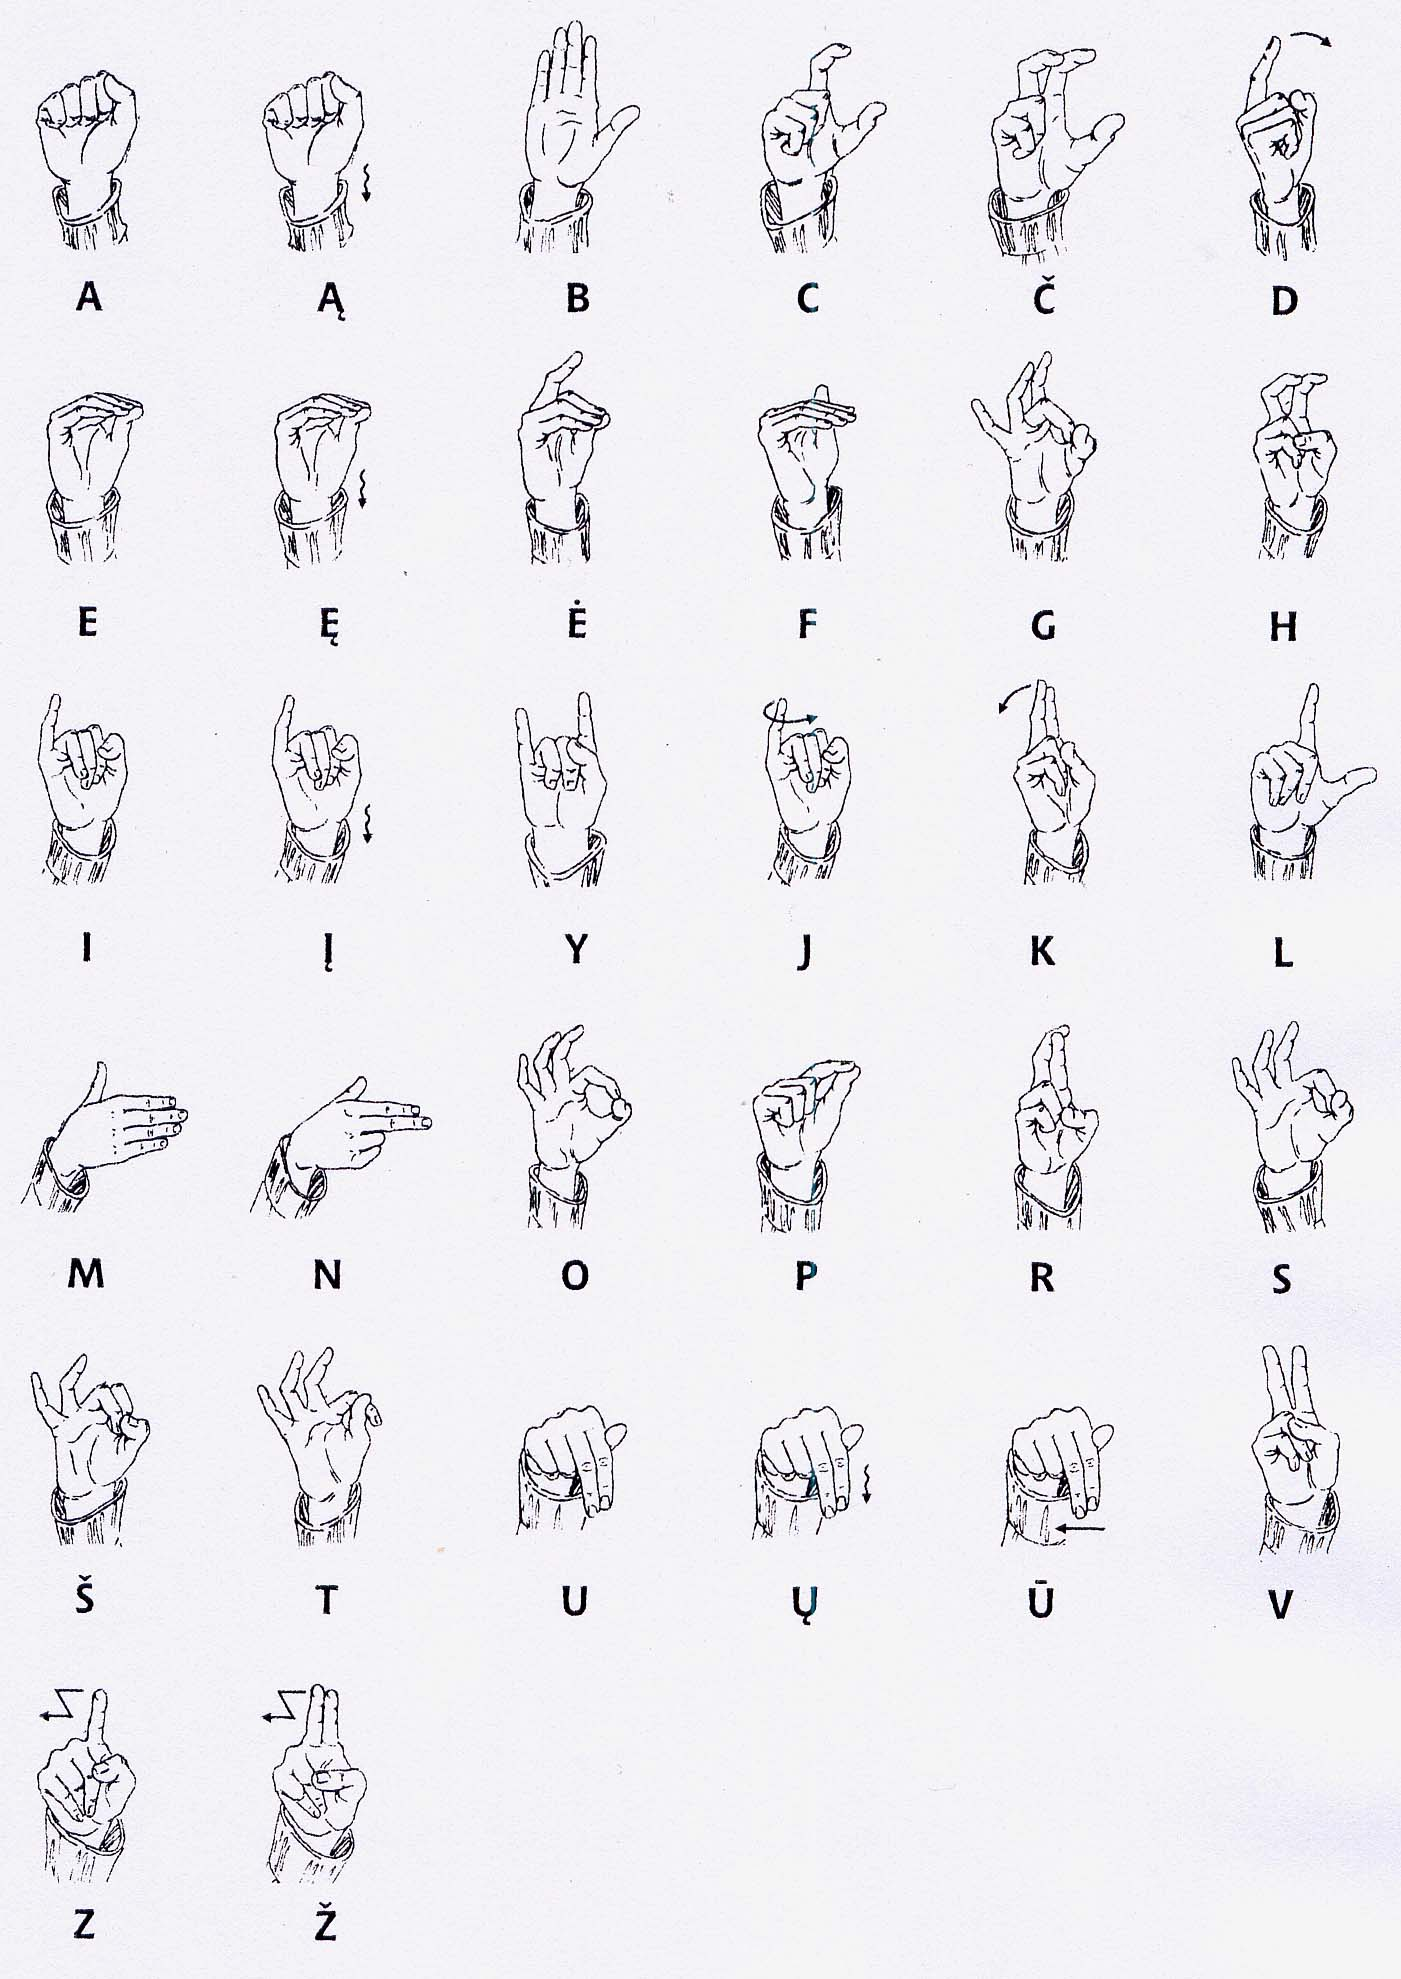
\includegraphics[scale=0.4]{img/lgk}
    \caption{Amerikiečių gestų kalbos abėcėlė}
    \label{img:lgk}
\end{figure}

	\item\textbf{Dinaminė gestų kalba} - tai žodžių lygio gestų kalba. Nesunku pastebėti, kad \ref{img:lgk} paveikslėlyje yra „Ą“, „D“, „Į“, „J“, „K“, „Ų“, „Z“ ar „Ž“ raidės, kurios priskiriamos dinaminių judesių klasei. Taip pat yra žodžių, kurie priskiriami statinei gestų kalbai dėl savo kilmės, taip ir yra raidžių, kurios priskiriamos dinaminei gestų kalbai. Dinaminiais judesiais yra išreiškiami įvairūs gestų kalbos žodžiai tokie, kaip, pavyzdžiui, LGK yra „labas“, „mano“ ar „vardas“ ar kiti.
	
	\item\textbf{Kitos ypatybės} - emocijos veide, liežuvis, burna ir kūno laikysena. Tai taip pat labai svarbios gestų kalbos ypatybės. Pavyzdžiui, klausiant gestų kalba klausimo, jei bus pakelti antakiai, tai reikš, kad laukiamas atsakymas „taip“ arba „ne“. Tačiau, jei antakiai bus suraukti, tai reikš, kad klausiama su paaiškinimu „kas“, „kur“, „kaip“ ar „ką“.
\end{enumerate}


\subsectionnonum{Darbo tikslas}
Išanalizuoti ir praktiškai išbandyti gestų kalbos vienetų atpažinimo galimybes iš video srauto.

\subsectionnonum{Darbo uždaviniai}
\begin{enumerate}
	\item Išanalizuoti konvoliucinius ir rekurentinius neuroninius tinklus bei jų panaudojimo būdus, gestų kalbos kontekste;
	\item Išsiaiškinti, kokie yra paruošti duomenų rinkiniai, kuriais naudojantis būtų galima apmokyti neuroninius tinklus;
	\item Sukurti neuroniais tinklais paremtą modelį gestų kalbos atpažinimui;
	\item Atlikti tyrimą ir nustatyti, kokiu tikslumu modeliai, skirti gestų atpažinimo uždaviniui, gali atpažinti lietuvių kalbos gestus iš video srauto;
\end{enumerate}

\subsectionnonum{Darbo eiga}
\begin{enumerate}
	\item Teorinės medžiagos analizė;
	\item Panašių ir jau įgyvendintų projektų paieška;
	\item Gestų kalbos video srautų paieška ir naujų vaizdo įrašų rengimas;
	\item Modelio apmokymai;
	\item Rezultatų palyginimai.
\end{enumerate}

\subsectionnonum{Panaudotos priemonės}
\begin{itemize}
	\item Python – programavimo kalba;
	\item TensorFlow – skirta darbui su apsimokančiomis sistemomis (\textit{angl. machine learning})
	\item Inception v3 – konvoliucinių neuroninių tinklų modelis;
	\item OpenCV – Python biblioteka darbui su vaizdais;
\end{itemize}


\section{Apsimokančios sistemos}
\textbf{Apsimokančios sistemos} (\textit{angl. machine learning}) – metodų rinkinys, kuris sugeba automatiškai analizuoti duomenų struktūras ir tuomet apdoroti nematytus modelius, kad prognozuotų duomenis arba priimtų sprendimus kitais būdais \cite{doi:10.1080/09332480.2014.914768}.

\subsection{Prižiūrimas mokymas}
\textbf{Prižiūrimas mokymas} (\textit{angl. supervised learning}) - tai apsimokančių sistemų apmokymo būdas, kuomet duomenys mokymui yra paruošiami taip, kad kiekvienas duomuo turėtų ir atitinkamą rezultatą. Kitaip tariant, jei yra duomuo $a$, tai yra ir jį atitinkantis rezultatas, arba dar vadinama etiketė (\textit{angl. label}) $b$. Tai būdas, kuris veikia medžio principu.

\begin{table}[H]\footnotesize
  \centering
  \caption{Pavyzdinis prižiūrimo mokymo apmokymui paruoštų duomenų rinkinys}
  {\begin{tabular}{| c | c | c | c | c | c || c |} \hline
    \thead{Nr.} & \thead{Pirštas nr. 1} & \thead{Pirštas nr. 2} & \thead{Pirštas nr. 3} & \thead{Pirštas nr. 4} & \thead{Pirštas nr. 5} & \thead{Raidė} \\
    \hline
    1. & Atlenktas & Užlenktas & Užlenktas & Užlenktas & Užlenktas & \thead{A} \\
    2. & Atlenktas & Atlenktas & Atlenktas & Atlenktas & Atlenktas & \thead{B} \\
    3. & Atlenktas & Sulenktas & Užlenktas & Užlenktas & Užlenktas & \thead{C} \\
    4. & Atlenktas & Sulenktas & Sulenktas & Užlenktas & Užlenktas & \thead{Č} \\
    5. & Sulenktas & Sulenktas & Sulenktas & Sulenktas & Sulenktas & \thead{E} \\
    6. & Atlenktas & Sulenktas & Sulenktas & Sulenktas & Sulenktas & \thead{F} \\
    \hline
  \end{tabular}}
  \label{tab:priziurimasPavyzdys}
\end{table}

\ref{tab:priziurimasPavyzdys} lentelėje pateikiamas pavyzdys su supaprastinta lietuvių gestų kalbos abėcėle. Lentelėje pateikiamos piršų padėtys, o pirštai numeruojami pagal \ref{appendix:pirstai} priede pateikiamą pirštų numeraciją. Kiekvieno piršto padėtis šiame pavyzdyje gali būti: \textit{atlenktas, sulenktas} ar \textit{užlenktas}. Ir kiekvienai padėčiai esant pateikiamas rezultatas, arba kitaip - etiketė, kokią raidę abėcėlėje atitinka pavaizduotos pirštų padėtys.


\begin{table}[H]\footnotesize
  \centering
  \caption{Pavyzdinė praktinė užduotis}
  {\begin{tabular}{| c | c | c | c | c | c || c |} \hline
    \thead{Nr.} & \thead{Pirštas nr. 1} & \thead{Pirštas nr. 2} & \thead{Pirštas nr. 3} & \thead{Pirštas nr. 4} & \thead{Pirštas nr. 5} & \thead{Raidė} \\
    \hline
    1. & Atlenktas & Sulenktas & Sulenktas & Sulenktas & Sulenktas & \thead{?} \\
    \hline
  \end{tabular}}
  \label{tab:priziurimasUzdavinys}
\end{table}

\ref{tab:priziurimasUzdavinys} lentelėje pateikiamas uždavinys, kuriame nurodoma ta pati informacija, kuri buvo pateikta \ref{tab:priziurimasPavyzdys} lentelėje, tačiau rezultatas nėra pateiktas, o jis randamas medžio principu.


\begin{figure}[H]
    \centering
    
\begin{forest}
  for tree={
    fit=band,% spaces the tree out a little to avoid collisions
  }
  [\textit{Pirštas nr. 4}
    [Atlenktas [\textbf{B}]]
    [Užlenktas
      [\textit{Pirštas nr. 3}
      	[Sulenktas [\textbf{Č}]]
	[Užlenktas
	  [\textit{Pirštas nr. 2}
	    [Užlenktas [\textbf{A}]]
	    [Sulenktas [\textbf{C}]]
	  ]
	]
      ]
    ]
    [Sulenktas
      [\textit{Pirštas nr. 1}
      	[Sulenktas [\textbf{E}]]
      	[Atlenktas [\textbf{F}]]
      ]
    ]  
  ]
\end{forest}
    \caption{Galimybių medis}
    \label{img:medis}
\end{figure}


Vien iš šio galimybių medžio galima matyti, kad pilnai užtenka sprendimui nustatyti 3 pirštų, kadangi rezultatų nėra daug. Jei būtų imama visa abėcėlės aibė, tuomet rezultato nustatymui būtų naudojama, galimai, visų pirštų padėtys.

\subsection{Neprižiūrimas mokymas}
\textbf{Neprižiūrimas mokymas} (\textit{angl. unsupervised learning}) - mokymas, kuomet duomenims nėra priskiriamos teisingos etiketės ar teisingi rezultatai. Pavyzdžiui, tai galėtų atitikti naujos kalbos mokymąsi be mokytojo ar bet kokio žodyno. Kuomet pastoviai matomas vis tas pats tekstas, žodžiai tampa atpažįstami, tačiau išversti jų neįmanoma. Tačiau tai nesukelia jokių nepatogumų, jei į tekstą reikia įrašyti tinkamą žodį, kuomet dėl daugybės duomenų yra aišku koks žodis su kokia galūne turėtų būti įrašytas.

\begin{table}[H]\footnotesize
  \centering
  \caption{Pavyzdinis neprižiūrimo mokymo apmokymui paruoštų duomenų rinkinys}
  {\begin{tabular}{| c | c | c | c | c | c |} \hline
    \thead{Nr.} & \thead{Pirštas nr. 1} & \thead{Pirštas nr. 2} & \thead{Pirštas nr. 3} & \thead{Pirštas nr. 4} & \thead{Pirštas nr. 5}  \\
    \hline
    1. & Atlenktas & Užlenktas & Užlenktas & Užlenktas & Užlenktas\\
    2. & Atlenktas & Atlenktas & Atlenktas & Atlenktas & Atlenktas \\
    3. & Atlenktas & Sulenktas & Užlenktas & Užlenktas & Užlenktas \\
    4. & Atlenktas & Sulenktas & Sulenktas & Užlenktas & Užlenktas \\
    5. & Sulenktas & Sulenktas & Sulenktas & Sulenktas & Sulenktas \\
    6. & Atlenktas & Sulenktas & Sulenktas & Sulenktas & Sulenktas \\
    \hline
  \end{tabular}}
  \label{tab:nepriziurimasPavyzdys}
\end{table}

\ref{tab:nepriziurimasPavyzdys} lentelėje pateikiamas pavyzdinis neprižiūrimam mokymui apmokyti paruoštų duomenų rinkinys. Duomenys tokie patys, kaip ir \ref{tab:priziurimasPavyzdys} lentelėje, tačiau nėra teisingo atsakymo sulpelio \textbf{„Raidė“}. Apmokius tokią sistemą būtent tokiais duomenimis vienas iš tikėtinų scenarijų, kur galima būtų panaudoti tokią sistemą, tai nuspėti, kokios raidės yra labiausiai tikėtinos ar tiesiog numatyti, kokia labiausiai tikėtina raidžių seka bus rodoma.


\subsection{Skatinamasis mokymas}
\textbf{Skatinamasis mokymas} (\textit{angl. reinforcement learning}) - labiausiai dirbtinį intelektą atitinkančių apsimokančių sistemų apmokymo modelis. Šis mokymas pagrįstas praktiniais bandymais. Kiekvienas teisingai gautas rezultatas yra būdas, kuriuo reikėtų sekti, ir kiekvienas blogai gautas rezultatas, yra būdas, kurio vertėtų atsisakyti. Dažniausiai šis apmokymo būdas naudojamas sistemą apmokant žaisti žaidimus. Vienas iš labiausiai žinomų būtent šiuo apmokymo būdu apmokytų modelių yra \textit{AlphaZero}, kuris sugeba laimėti prieš pasaulio šachmatų čempionus. Tai puikus pavyzdys to, kaip kompiuteris iš laimėjimų, už kuriuos gauna taškus, ir pralaimėjimų, už kuriuos jam taškai atimami, sugeba rasti laimėjimo strategijas kiekviename žingsnyje ir taip, nuolatos tobulėdamas, laimėti dvikovas ar apskritai spręsti uždavinius, kuriuose reikalingas pastabumas ir strategijų kūrimas.


\section{Neuroniniai tinklai}
Žmogaus smegenys yra labai sudėtingas, netiesinis ir paralelinis kompiuteris \cite{Hay09}. Kiekvieno žmogaus kūnas yra sudarytas iš milijardų nervinių ląstelių vadinamų neuronais. Jie sukuria ir/arba perduoda elektrocheminius impulsus. Neuronai tarpusavyje yra sujungti dendritais, ant kurių yra sinapsės. 

Kiekvienas sužadintas neuronas dėl pasikeitusios temperatūros, spaudimo, skausmo ar kitų veiksnių, perduoda informaciją į smegenis dėl sprendimo, ką daryti, priėmimo. Neuronų paskirtis - siųsti signalą iš vieno neurono į kitą, kol galiausiai signalas pasiekia smegenis. Svarbu ir tai, kad kiekvienas neuronas yra nepriklausomas nuo kito. Tai tik grandis, kuri yra atsakinga už signalo priėmimą ir perdavimą. Smegenims gavus signalą, jį apdorojus ir priėmus sprendimą, signalas tuo pačiu keliu siunčiamas atgal, kol pirmąjį sužadinimą gavęs neuronas sulaukia atsakymo. 

\subsection{Perceptronas}

Parceptronas (\textit{angl. perceptron}) – kompiuterinis modelis, skirtas atkartoti žmogaus kūne esančių neuronų darbą. Jis, kaip ir neuronas, gali gauti vieną ar kelias įeigas ir generuoti vieną išeigą. Neuronas yra skirtas tik perduoti impulsą, o perceptronas pritaiko aktyvacijos funkciją. Šis skirtumas tarp neurono ir perceptrono yra todėl, kad žmogus turi smegenis, o perceptronas atlieka smegenų vaizdinį. Toliau pateikiamas perceptrono pavyzdys.

\begin{figure}[H]
	\centering
	\tikzset{%
		every neuron/.style={
			circle,
			draw,
			minimum size=1cm
		},
	}
	
	\begin{tikzpicture}[x=1.5cm, y=1.5cm, >=stealth]
	\centering
	
	\foreach \m/\l [count=\y] in {1,2,3,4}
	\node [every neuron/.try, neuron \m/.try] (input-\m) at (0,2.5-\y) {};
	
	\foreach \m [count=\y] in {1,2,3,4}
	\node [every neuron/.try, neuron \m/.try ] (weight-\m) at (2,2.5-\y) {};
	
	\foreach \m [count=\y] in {1}
	\node [every neuron/.try, neuron \m/.try ] (sum-\m) at (4,1.6-\y*1.6) {};
	
	\foreach \m [count=\y] in {1}
	\node [every neuron/.try, neuron \m/.try ] (funk-\m) at (6,1.6-\y*1.6) {};
	
	\foreach \m [count=\y] in {1}
	\node [every neuron/.try, neuron \m/.try ] (output-\m) at (8,1.6-\y*1.6) {};
	
	\foreach \i in {1,...,4}
	\draw [->] (input-\i) -- (weight-\i);
	
	\foreach \i in {1,...,4}
	\draw [->] (weight-\i) -- (sum-1);
	
	\draw [->] (sum-1) -- (funk-1);
	
	\draw [->] (funk-1) -- (output-1);
	
	\foreach \l [count=\x from 0] in {Įeigos\\, Svoriai\\, Suma\\, Aktyvacijos\\funkcija, Išeiga\\}
	\node [align=center, above] at (\x*2,2) {\l};
	
	
	\draw (0,1.49) node {$i_1$};
	\draw (0,0.49) node {$i_2$};
	\draw (0,0.045) node {$\vdots$};
	\draw (0,-0.51) node {$i_n$};
	\draw (0,-1.51) node {$1$};
	
	\draw (2,1.49) node {$w_1$};
	\draw (2,0.49) node {$w_2$};
	\draw (2,0.045) node {$\vdots$};
	\draw (2,-0.51) node {$w_n$};
	\draw (2,-1.51) node {$b$};
	
	\draw (4,0) node {$\sum$};
	
	\draw (6,0) node {$f(x)$};
	
	\draw (8,0) node {$o_i$};
	\end{tikzpicture}
	\caption{Perceptrono pavyzdys} \label{fig:perceptron}
\end{figure}

\ref{fig:perceptron} paveikslėlyje pavaizduotame pavyzdyje esančią išeigą galima aprašyti formule:
\begin{equation}
	o_i = f((\sum_{j=0}^{n}i_j \cdot w_j) + 1 \cdot b)
	\label{eq:perceptron}
\end{equation}

\ref{eq:perceptron} formulėje $i_j$ - $j$-toji įeiga, $w_j$ - $j$-tosios įeigos svorinis koeficientas, $b$ - poslinkio koeficientas, kuris dažniausiai kaip įeigos vertę turi $1$.

Kiekvienas perceptronas gali gauti vieną ar kelias įeigas (\textit{angl. input}). Visų šių įeigų svorių suma yra sudedama ir paskui apdorojama aktyvacijos funkcija. Pritaikius aktyvacijos funkciją yra gaunama išeiga (\textit{angl. output}). Yra keletas skirtingų aktyvacijos funkcijų. Pačios populiariausios pateikiamos \ref{fig:aktyvacijosfunkc} diagramoje.
\begin{figure}[H]
	\centering
	
	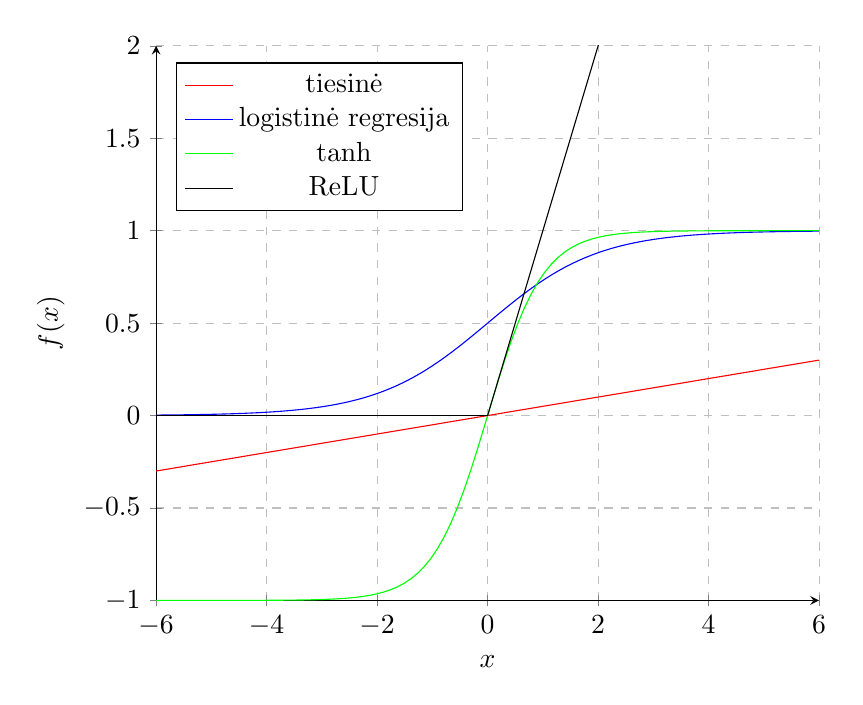
\begin{tikzpicture}
	\begin{axis}[
	axis lines = left,
	width=10cm,
	xlabel = $x$,
	ylabel = {$f(x)$},
	ymax = 2,
	ymajorgrids=true,
	xmajorgrids=true,
	legend pos=north west,
	grid style=dashed,
	]
	%Below the red parabola is defined
	\addplot [
	domain=-6:6, 
	samples=100, 
	color=red,
	]
	{0.05*x};
	\addlegendentry{tiesinė}
	%Here the blue parabloa is defined
	\addplot [
	domain=-6:6,
	samples=100, 
	color=blue,
	]
	{1/(1+exp(-x))};
	\addlegendentry{logistinė regresija}
	
	\addplot [
	domain=-6:6,
	samples=100, 
	color=green,
	]
	{tanh(x)};
	\addlegendentry{tanh}
	
	
	\addplot [
	domain=0:6,
	samples=100, 
	color=black,
	]
	{x};
	\addlegendentry{ReLU}
	
	
	\addplot [
	domain=-6:0,
	samples=100, 
	color=black,
	]
	{0};
	
	\end{axis}
	\end{tikzpicture}
	
	\caption{Aktyvacijos funkcijos} \label{fig:aktyvacijosfunkc}
\end{figure}


\ref{fig:aktyvacijosfunkc} diagramoje pateikiamos šios funkcijos:

\begin{itemize}
	\item Tiesinė – $f(x) = a \cdot x$;
	\item Logistinės regresijos – $f(x) = \frac{1}{1+e^{-x}}$;
	\item Tanh – $f(x) = \tanh(x) = \frac{2}{1+e^{-2x}} - 1$;
	\item ReLU – $f(x) = \begin{cases}
	0 & \text{, kai } x < 0 \\
	x & \text{, kai } x \ge 0
	\end{cases} $.
\end{itemize}

\subsection{Daugiasluosknis perceptronas}

\textbf{Daugiasluoksnis perceptronas} (\textit{angl. multilayer perceptron}) – struktūra, sudaryta iš kelių sluoksnių perceptronų. 

Dažniausiai daugiasluoksnis perceptronas turi tris ar daugiau sluoksnius – įeigos (\textit{input layer}), paslėptąjį (\textit{hidden layer}) ir išeigos (\textit{output layer}). Svarbu pastebėti, kad paslėptajame sluoksnyje gali būti daugiau nei vienas sluoksnis. Daugiasluoksnis perceptronas kaip aktyvacijos funkciją naudoja nelinijines aktyvacijos funkcijas. Dažniausiai tai būna \textit{tanh} ar loginės regresijos funkcijos. Kiekvienas sluoksnio elementas yra sujungtas su kito sluoksnio elementu, todėl tai sudaro pilnai apjungtą (\textit{angl. fully connected}) tinklą. Yra pavyzdžių, kur daugiausluoksniai perceptronai naudojami atpažinti žodinę kalbą ar versti tekstus. 

Toliau pateikiamas daugiasluoksnio perceptrono pavyzdys.

\begin{figure}[H]
	\centering
	\tikzset{%
		every neuron/.style={
			circle,
			draw,
			minimum size=1cm
		},
	}
	
	\begin{tikzpicture}[x=1.5cm, y=1.5cm, >=stealth]
	\centering
	
	\foreach \m/\l [count=\y] in {1,2,3}
	\node [every neuron/.try, neuron \m/.try] (input-\m) at (0,1.9-\y) {};
	
	\foreach \m [count=\y] in {1,2,3,4}
	\node [every neuron/.try, neuron \m/.try ] (hidden-\m) at (2,2.5-\y) {};
	
	\foreach \m [count=\y] in {1,2}
	\node [every neuron/.try, neuron \m/.try ] (output-\m) at (4,2.3-\y*1.6) {};
	
	\foreach \i in {1,...,3}
	\foreach \j in {1,...,4}
	\draw [->] (input-\i) -- (hidden-\j);
	
	\foreach \i in {1,...,4}
	\foreach \j in {1,...,2}
	\draw [->] (hidden-\i) -- (output-\j);
	
	\foreach \l [count=\x from 0] in {Įeigos, Paslėptasis, Išeigos}
	\node [align=center, above] at (\x*2,2) {\l \\ sluoksnis};
	\end{tikzpicture}
	\caption{Daugiasluoksnio perceptrono pavyzdys} \label{fig:multilayer}
\end{figure}



\subsection{Dirbtiniai neuroniniai tinklai}
\textbf{Dirbtiniai neuroniniai tinklai} (\textit{angl. artificial neural networks}) – struktūra, sukurta remiantis žmogaus nervinės sistemos darbu. Dirbtiniai neuroniniai tinklai gali būti išmokinti atlikti klasifikavimo, spėjimo, sprendimų priėmimo ir kitas užduotis.


Dirbtiniai neuroniniai tinklai remiasi daugiasluoksnio perceptrono principu ir susideda iš šių sluoksnių - įeigos, paslėptojo, kuris gali būti sudarytas iš kelių sluoksnių, ir išeigos.

\subsection{Konvoliuciniai neuroniniai tinklai}

\textbf{Konvoliuciniai neuroniniai tinklai} (\textit{angl. convoliutional neural networks}) – specialios rūšies vienpusiai (\textit{angl. feed-forward}) neuroniniai tinklai, kurie remiasi daugiasluoksnio perceptrono principu. Šie tinklai, kurie remiasi \textit{ReLU} principu yra kelis kartus greitesni, nei tie, kurie remiasi kitais principais, pavyzdžiui, \textit{tanh} \cite{NIPS2012_4824}. 

Toliau aptariami keli pagrindiniai konvoliucinių neuroninių tinklų sluoksniai.

\subsubsection{Konvoliucinis sluoksnis}

\textbf{Konvoliucinis sluoksnis} (\textit{angl. convoliution layer}) – sluoksnis, skirtas išskirti savybes. Šio sluoksnio 
pritaikymą galima skaidyti į tokias operacijas:


\begin{enumerate}
	\item \textbf{Įeiga}, susidedanti iš $ W_1 \times H_1 \times D_1 $, kur $ W_1 $ - plotis, $ H_1 $ - aukštis ir $ D_1 $ - gylis;
	\item \textbf{Parametrai}, kurie susideda iš $ F $, $ K $, $ P $ ir $ S $, kur:
	\begin{itemize}
		\item $ F $ - filtro dydis (dažniausiai taikomas $ 3 \times 3 $ filtras);
		\item $ K $ - filtrų skaičius (dažniausiai naudojamas  $ 2^n $, kur $ n $ - natūralusis skaičius);
		\item $ P $ - papildomas rėmelis matricai, sudarytas iš 0. Dažniausiai naudojama $ M = \frac{F - 1}{2} $, kur $ M $ yra iš kiekvienos matricos pusės pridedamų eilučių ar stulpelių skaičius, sudarytas iš $0$, tam, kad matrica nepakeistų savo dydžio po šio sluoksnio pritaikymo; 
		\item $ S $ - žingsnis, per kiek paslenkamas filtras (dažniausiai naudojamas $ 1 $);
	\end{itemize}
	\item \textbf{Išeiga}, susidedanti iš $ W_2 \times H_2 \times D_2 $, kur $ W_2 = \frac{W_1 - F + 2P}{S} + 1 $ - plotis, $ H_2 = \frac{H_1 - F + 2P}{S} + 1 $ - aukštis ir $ D_2 = K $ - gylis
\end{enumerate}

\begin{table}[H]\footnotesize
	\centering
	\caption{Pavyzdinės konvoliucinio sluoksnio užduoties ypatybės}
	{\begin{tabular}{| c | c | c | c | c | c | c | c | c | c |} 
		\hline
		\multicolumn{3}{| c |}{\thead{Įeiga}} &
		\multicolumn{4}{ c |}{\thead{Parametrai}} & \multicolumn{3}{ c |}{\thead{Išeiga}} \\
		\hline
		$W_1$ & $H_1$ & $D_1$ & $F$ & $K$ & $P$ & $S$ & $W_2$ & $H_2$ & $D_2$  \\
		\hline
		3 & 3 & 1 & 3 $\times$ 3 & 1 & 1 & 1 & 3 & 3 & 1 \\
		\hline
	\end{tabular}}
	\label{tab:convT}
\end{table}
	
Toliau, \ref{eq:convl} formulėje pateikiamas pavyzdys, kuriame naudojamos \ref{tab:convT} lentelėje pateiktos pavyzdinės konvoliucinio sluoksnio užduoties ypatybės. Spalvos šioje formulėje žymi skirtingų matricų elementus, kur geltona - įeigos matricos elementų spalva, raudona - papildomo rėmelio $P$ spalva, mėlyna - filtro matricos spalva, o žalia - išeigos matricos elemento spalva. \ref{eq:convl1} ir \ref{eq:convl2} formulėse pateikiami konkretūs pavyzdžiai, kuriais remiantis buvo gautos \ref{eq:convl} formulės reikšmės.

\begin{equation}\label{eq:convl}
\begin{bmatrix}
\textcolor{myyellow}{1} & \textcolor{myyellow}{8} & \textcolor{myyellow}{6} \\
\textcolor{myyellow}{9} & \textcolor{myyellow}{2} & \textcolor{myyellow}{4} \\
\textcolor{myyellow}{3} & \textcolor{myyellow}{7} & \textcolor{myyellow}{5}
\end{bmatrix}
\cdot
\begin{bmatrix}
\textcolor{myblue}{1} & \textcolor{myblue}{0} & \textcolor{myblue}{1} \\
\textcolor{myblue}{0} & \textcolor{myblue}{1} & \textcolor{myblue}{0} \\
\textcolor{myblue}{1} & \textcolor{myblue}{0} & \textcolor{myblue}{1}
\end{bmatrix}
=
\begin{bmatrix}
\textcolor{mygreen}{3} & \textcolor{mygreen}{21} & 8 \\
24 & 17 & 19 \\
5 & 20 & 7
\end{bmatrix}
\end{equation}

\begin{equation}\label{eq:convl1}
\textcolor{myred}{0} \cdot \textcolor{myblue}{1}+\textcolor{myred}{0} \cdot \textcolor{myblue}{0}+\textcolor{myred}{0} \cdot \textcolor{myblue}{0}+\textcolor{myred}{0} \cdot \textcolor{myblue}{0}+\textcolor{myyellow}{1} \cdot \textcolor{myblue}{1}+\textcolor{myyellow}{8} \cdot \textcolor{myblue}{0}+\textcolor{myred}{0} \cdot \textcolor{myblue}{1}+\textcolor{myyellow}{9} \cdot \textcolor{myblue}{0}+\textcolor{myyellow}{2} \cdot \textcolor{myblue}{1}=\textcolor{mygreen}{3}
\end{equation}


\begin{equation}\label{eq:convl2}
\textcolor{myred}{0} \cdot \textcolor{myblue}{1}+\textcolor{myred}{0} \cdot \textcolor{myblue}{0}+\textcolor{myred}{0} \cdot \textcolor{myblue}{1}+\textcolor{myyellow}{1} \cdot \textcolor{myblue}{0}+\textcolor{myyellow}{8} \cdot \textcolor{myblue}{1}+\textcolor{myyellow}{6} \cdot \textcolor{myblue}{0}+\textcolor{myyellow}{9} \cdot \textcolor{myblue}{1}+\textcolor{myyellow}{2} \cdot \textcolor{myblue}{0}+\textcolor{myyellow}{4} \cdot \textcolor{myblue}{1}=\textcolor{mygreen}{21}
\end{equation}

\subsubsection{Telkimo sluoksnis}

\textbf{Telkimo sluoksnis} (\textit{angl. pooling layer}) – sluoksnis, skirtas sumažinti matricą, paliekant tik svarbiausias jos dalis. Dažniausiai naudojamos vidutinės (\textit{angl. average pooling}) arba didžiausios (\textit{angl. max pooling}) reikšmės operacijos. 

Telkimo sluoksnio operacijas galima skaidyti į tokias dalis:

\begin{enumerate}
	\item \textbf{Įeiga}, susidedanti iš $ W_1 \times H_1 \times D_1 $, kur $ W_1 $ - plotis, $ H_1 $ - aukštis ir $ D_1 $ - gylis
	\item \textbf{Parametrai}, kurie susideda iš $ F $ ir $ S $, kur $ F $ - filtro dydis (dažniausiai taikomas $ 2 \times 2 $ filtras) ir $ S $ - žingsnis, per kiek paslenkamas filtras (dažniausiai naudojamas $ 2 $)
	\item \textbf{Išeiga}, susidedanti iš $ W_2 \times H_2 \times D_2 $, kur $ W_2 = \frac{W_1 - F}{S} + 1 $ - plotis, $ H_2 = \frac{H_1 - F}{S} + 1 $ - aukštis ir $ D_2 = D_1 $ - gylis
\end{enumerate}


\begin{table}[H]\footnotesize
	\centering
	\caption{Pavyzdinės telkimo sluoksnio užduoties ypatybės}
	{\begin{tabular}{| c | c | c | c | c | c | c | c |} 
		\hline
		\multicolumn{3}{| c |}{\thead{Įeiga}} &
		\multicolumn{2}{ c |}{\thead{Parametrai}} & \multicolumn{3}{ c |}{\thead{Išeiga}} \\
		\hline
		$W_1$ & $H_1$ & $D_1$ & $F$ & $S$ & $W_2$ & $H_2$ & $D_2$  \\
		\hline
		4 & 4 & 1 & 2 $\times$ 2 & 2 & 3 & 3 & 1 \\
		\hline
	\end{tabular}}
	\label{tab:pollT}
\end{table}	
Toliau, \ref{eq:poll} formulėje pateikiamas pavyzdys, kuriame naudojamos \ref{tab:pollT} lentelėje pateiktos pavyzdinės telkimo sluoksnio užduoties ypatybės. Spalvos šioje formulėje žymi filtro su žingsniu pritaikytas operacijas gauti išeigai. \ref{eq:poll1} ir \ref{eq:poll2} formulėse pateikiami konkretūs pavyzdžiai, kuriais remiantis buvo gautos \ref{eq:poll} formulės reikšmės.

\begin{equation}\label{eq:poll}\def\y{\color{myyellow}}\def\b{\color{myblue}}\def\r{\color{myred}}\def\g{\color{mygreen}}
\begin{bmatrix}
\y{1} & \y{3} & \b{1} & \b{3} \\
\y{2} & \y{5} & \b{4} & \b{2} \\
\g{4} & \g{3} & \r{2} & \r{5} \\
\g{2} & \g{5} & \r{4} & \r{2} \\
\end{bmatrix}
= 
\begin{bmatrix}
\y{5} & \b{4} \\
\g{5} & \r{5} 
\end{bmatrix}
\end{equation}
\begin{equation}\label{eq:poll1}
max(
\begin{bmatrix}
\textcolor{myyellow}{1} & \textcolor{myyellow}{3} \\
\textcolor{myyellow}{2} & \textcolor{myyellow}{5}
\end{bmatrix}
) = \textcolor{myyellow}{5}
%1, 3, 1, 3, 2, 5, 2, 4, 3
\end{equation}
\begin{equation}\label{eq:poll2}
max(
\begin{bmatrix}
\textcolor{myblue}{1} & \textcolor{myblue}{3} \\
\textcolor{myblue}{4} & \textcolor{myblue}{2} 
\end{bmatrix}
) = \textcolor{myblue}{4}
\end{equation}

\subsubsection{Atsisakymo sluoksnis}
\textbf{Atsisakymo sluoksnis} (\textit{angl. dropout layer}) – konvoliucinių tinklų sluoksnis, skirtas normalizuoti ir sureguliuoti tarpusavyje susijusių neuronų sąryšius, skirtus perduoti signalus. Mokymo fazėje dažniausiai ištrinamos neuronuose esančios reikšmės tam, kad šis per naują apsimokytų. Galimai netgi atsisakoma tam tikrų neuronų darbo \cite{DBLP:journals/corr/abs-1207-0580}.

\begin{figure}[H]
	\centering
	
	\begin{minipage}{.4\textwidth}
		\centering
		\tikzset{%
			every neuron/.style={
				circle,
				draw,
				minimum size=0.5cm
			},
		}
		
		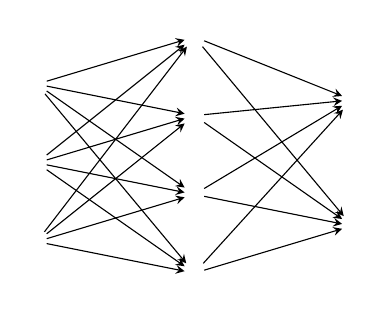
\begin{tikzpicture}[x=1cm, y=1cm, >=stealth]
		\centering
		
		\foreach \m/\l [count=\y] in {1,2,3}
		\node [every neuron/.try, neuron \m/.try] (input-\m) at (0,1.9-\y) {};
		
		\foreach \m [count=\y] in {1,2,3,4}
		\node [every neuron/.try, neuron \m/.try ] (hidden-\m) at (2,2.5-\y) {};
		
		\foreach \m [count=\y] in {1,2}
		\node [every neuron/.try, neuron \m/.try ] (output-\m) at (4,2.3-\y*1.6) {};
		
		\foreach \i in {1,...,3}
		\foreach \j in {1,...,4}
		\draw [->] (input-\i) -- (hidden-\j);
		
		\foreach \i in {1,...,4}
		\foreach \j in {1,...,2}
		\draw [->] (hidden-\i) -- (output-\j);
		
		\end{tikzpicture}
		\caption{Standartinis neuroninis tinklas} \label{fig:snn}
	\end{minipage}
	\begin{minipage}{.4\textwidth}
		\centering
		\tikzset{%
			every neuron/.style={
				circle,
				draw,
				minimum size=0.5cm
			},
			cross/.style={cross out, draw=black, minimum size=2*(#1-\pgflinewidth), inner sep=0pt, outer sep=0pt},
			%default radius will be 1pt. 
			cross/.default={0.19cm},
		}
		
		\begin{tikzpicture}[x=1cm, y=1cm, >=stealth]
		\centering
		
		\foreach \m/\l [count=\y] in {1,2,3}
		\node [every neuron/.try, neuron \m/.try] (input-\m) at (0,1.9-\y) {};
		
		\foreach \m [count=\y] in {1,2,3,4}
		\node [every neuron/.try, neuron \m/.try ] (hidden-\m) at (2,2.5-\y) {};
		
		\foreach \m [count=\y] in {1,2}
		\node [every neuron/.try, neuron \m/.try ] (output-\m) at (4,2.3-\y*1.6) {};
		
		\foreach \i in {1,3}
		\foreach \j in {1,3}
		\draw [->] (input-\i) -- (hidden-\j);
		
		\foreach \i in {1,3}
		\foreach \j in {1,...,2}
		\draw [->] (hidden-\i) -- (output-\j);
		
		\draw (0,-0.1) node[cross] {};
		
		\draw (2,0.5) node[cross] {};
		
		\draw (2,-1.5) node[cross] {};
		\end{tikzpicture}
		\caption{Tinklas po atsisakymo sluoksnio} \label{fig:sdnn}
	\end{minipage}
\end{figure}


\subsection{Rekurentiniai neuroniniai tinklai}

\textbf{Rekurentiniai neuroniniai tinklai} (\textit{angl. recurrent neural networks}) – vienpusiai neuroniniai tinklai, kurie remiasi daugiasluoksnio perceptrono principu. Šie tinklai, apima kitų laiko vienetų apdorotą informaciją ir bendrą kitimą laike \cite{DBLP:journals/corr/Lipton15}.


\begin{figure}[H]
	\centering
	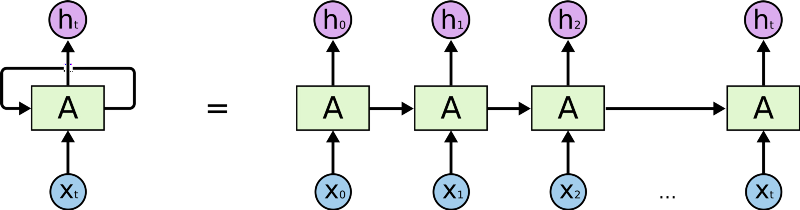
\includegraphics[scale=0.4]{img/rnn}
	\caption[]{Rekurentinių neuroninių tinklų veikimo principas\footnotemark}
	\label{img:RNT}
\end{figure}
\footnotetext{\url{https://cdn-images-1.medium.com/max/1600/0*WdbXF_e8kZI1R5nQ.png}}

\ref{img:RNT} paveiksėlyje yra pavaizduotas bendrinis rekurentinių neuroninių tinklų veikimo principas, kurį galima užrašyti formule:

\begin{equation}\label{eq:RNT}
h_t = f_w(h_{t-1}, x_t)
\end{equation}

Kur $h_t$ - paslėpto sluoksnio būsena laiko momentu $t$, kurią dar būtų galima vadinti $t$ žingsnio išeiga, $f_w$ - aktyvacijos funkcija $f$ su parametrais $w$, $h_{t-1}$ - praėjusio žingsnio būsena, o $x_t$ - įeigos vektorius. Iš šios formulės galima pastebėti, kad kiekviena būsena gauna praeito žingsnio būsena, kuri yra reikalinga norint stebėti būsenas kintant laike	.


\subsubsection{Rekurentinių neuroninių tinklų tipai}

\begin{figure}[H]
	\centering
	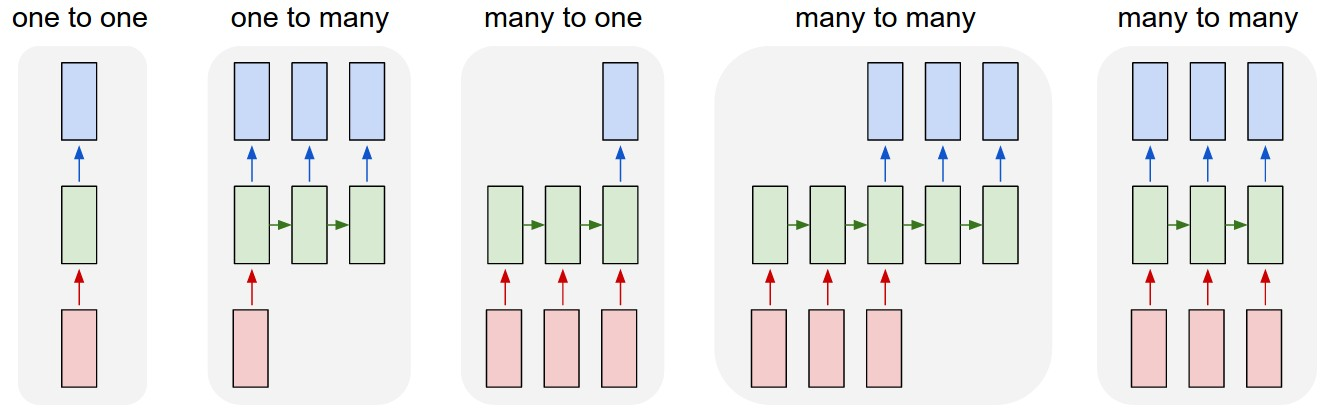
\includegraphics[scale=0.3]{img/nn-tipai}
	\caption[]{Rekurentinių neuroninių tinklų tipai\footnotemark}
	\label{img:tipai}
\end{figure}
\footnotetext{\url{https://discuss.pytorch.org/uploads/default/original/1X/6415da0424dd66f2f5b134709b92baa59e604c55.jpg}}

\ref{img:tipai} paveikslėlyje pavaizduoti keturi skirtingi būdai, kuriais naudojantis rekurentiniai neuroniniai tinklai veikia. Rausvos spalvos kvadratėlis reiškia įeigą, žalsvas - paslėptuosius sluoksnius, o melsvas - išeigą. Pateikiami šie būdai:

\begin{itemize}
	\item \textbf{Vienas su vienu} (\textit{angl. one to one}) – būdas, kuriame yra viena įeiga, paslėptasis sluoksnis ir išeiga. Šis būdas dažniausiai taikomas konstruojant konvoliucinius neuroninius tinklus. Kaip pavyzdį galima pateikti paveikslėlio atpažinimą. Tai galėtų būti statinės gestų kalbos atpažinimas.
	\item \textbf{Vienas su daug} (\textit{angl. one to many}) – būdas, kuriame yra viena įeiga ir kelios išeigos. Vienas iš panaudojimo būdų galėtų būti sakinio suformavimas iš paveikslėlio. Toks tinklas ne tik atpažįsta pagrindinį objektą kadre, bet ir apibūdina esančią aplinką, daro kitus sprendimus;
	\item \textbf{Daug su vienu} (\textit{angl. many to one}) – būdas, kuriame yra daug įeigų, bet tik viena išeiga. Tokio būdo pavyzdys galėtų būti vieno žodžio, tarkime, „labas“ atpažinimas iš video srauto.
	\item \textbf{Daug su daug} (\textit{angl. many to many}) – būdas, kuriame yra daug įeigų ir daug išeigų. Šis būdas gali būti skaidomas į dvi dalis:
	\begin{itemize}
		\item \textbf{Priklausomas} - įeigų skaičius sutampa su išeigų skaičiumi. Kiekviena įeiga turi savo išeigos atitikmenį. Tai būtų dalinai galima gretitinti su \textit{vienas su vienu} būdu.
		\item \textbf{Nepriklausomas} - įeigos skaičius galimai nesutampa su išeigų skaičiumi. Kiekviena įeiga yra nepriklausoma ir išeigos dėliojamos pagal tam tikrus aspektus. Tokio būdo pavyzdys galėtų būti neuroniniai tinklai, kurie atlieka vertėjo funkcijas, pavyzdžiui, iš anglų į lietuvių kalbas, nes skiriasi tiek gramatika, tiek sakinių stilistika. Šis būdas taip pat galėtų būti pritaikomas versti gestų kalbą.
	\end{itemize}
\end{itemize}

\subsubsection{Rekurentinių neuroninių tinklų modeliai}

Viena pagrindinių problemų, su kuria susiduria paprastieji rekurentiniai neuroniniai tinklai yra nykstančių gradientų problema (\textit{angl. vanishing gradient problem}). Tai problema, kurios metu kiekvieno laiko momentu perceptronas apskaičiuoja naujas reiškmes iš praeitame žingsnyje turimų duomenų ir kaip įeiga priima praeito laiko momento išeigą. 

\begin{equation}
	f(w_n \cdot h_n)=h_{n+1}
\end{equation}

Šioje formulėje $w_n$ - $n$-tojo sluoksnio svoris, $h_n$ - $n$-tojo sluoksnio paslėptoji būsena, o $f(x)$ - aktyvacijos funkcija.

Tinklo pabaigoje gaunamas praradimas (\textit{angl. loss}) arba kitaip - skirtumas tarp to, kas turėjo būti gauta ir ką tinklas gauna. Sakysime, kad $f(h_n)$ bus funkcija $f$, kurios parametras $h_n$ yra paskutinio sluoksnio paslėptoji būsena.

Norint pakeisti $w_n$ ($n$-tojo elemento svorį), tai galima padaryti apskaičiuojant gradientą atsižvelgiant į $w_n$.

\begin{equation}
	\frac{\partial Loss}{\partial w_n} = \frac{\partial Loss}{\partial f(h_n)} \cdot \frac{\partial f(h_n)}{\partial w_n} = \frac{\partial Loss}{\partial f(h_n)} \cdot f'(h_n) \cdot w_n
\end{equation}

Čia $\frac{\partial Loss}{\partial f(h_n)}$ yra dalinė išvestinė to, kaip skaičiuojamas praradimas. Svarbu tai, kad jis skaičiuojamas iš $f(h_n)$, todėl tai bus pastovi grįžtamojo ryšio (\textit{angl. backpropagation}) lygtis.

Tęsiant toliau, pirmojo svorio $w_1$ reikšmę galima apskaičiuoti pagal šią lygtį:

\begin{equation}
\frac{\partial Loss}{\partial w_1} = \frac{\partial Loss}{\partial f(h_n)} \cdot \frac{\partial f(h_n)}{\partial h_{n-1}} \cdots \frac{\partial f(h_2)}{\partial h_1} \cdot \frac{\partial f(h_1)}{\partial w_1} = \frac{\partial f(Loss)}{\partial f(h_n)} \cdot f'(h_n) \cdot w_n \cdots f'(h_1) * w_1
\end{equation}

Dėl šios priežasties ilgainiui dėl per naują skaičiuojamų svorių, perceptronas susiduria su problema, kad „pamiršta“, kas buvo prieš daugiau nei vieną laiko momentą - $w_1$ palaipsniui pradeda nebekisti dėl ilgų skaičiavimų ir tampa labai mažas. Tai reiškia, kad rekurentiniai neuroniniai tinklai paprasčiausiai vadovaujasi trumpalaikės atminties principu. Dėl šios priežasties buvo sukurtos keletas architektūrų, kurios sugebėtų atsiminti ir teisingai įvertinti esamą situaciją. Toliau pateikiama dažniausiai šiuo metu naudojamos RNT architektūros spręsti šią problemą.

\subsubsubsection{LSTM}
1997 metais Hochreiter ir Schmidhuber pristatė LSTM modelį, kuris, buvo manyta, galės išspręsti nykstančiųjų gradientų problemą. Šis modelis ypatingas tuo, jog kiekvienas įprastas paslėptojo sluoksnio mazags (\textit{angl. node}) yra pakeistas atminties ląstele \cite{DBLP:journals/corr/Lipton15}.

\textbf{LSTM} – ilga trumpalaikė atmintis (\textit{angl. long short-term memory}) - RNT architektūra, kuri sugeba atsiminti informaciją ilgesniam laiko tarpui. 

Paprasti RNT priima buvusią paslėptąją būseną, pritaiko aktyvacijos funkciją ir grąžina naują būseną. LSTM daro beveik tą patį, tik priima dar ir savo buvusią būseną ir grąžina savo naują būseną. 

LSTM įveda naują sąvoką - vartai (\textit{angl. gate}). LSTM turi trijų skirtingų tipų vartus:

\begin{itemize}
	\item \textbf{Užmaršties vartai} (\textit{angl. forget gate}) - juose apdorojama praeita paslėptoji būsena ir dabartinė įeiga. Šių vartų išeiga - nuosprendis, ką vertėtų pasilikti ląstelės būsenoje, o ką - užmiršti. Kuo vertė artimesnė 1 - tuo tai labiau verta atsiminti, o arčiau 0 - pamiršti;
	\item \textbf{Įeigos vartai} (\textit{angl. input gate}) - įeigos funkcija atnaujina ląstelės būseną;
	\item \textbf{Išeigos vartai} (\textit{angl. output gate}) nusprendžia, kurios ląstelės būsenos reikšmės bus pridedamas į paslėptąją būseną, kuri bus visos ląselės išeiga. Taip pat labai svarbu paminėti ir faktą, kad pasiliekamos ir tos reikšmės ar būsenos, kurios manoma, kad bus reikalingos ateityje.
\end{itemize}

\begin{figure}[H]
	\centering
	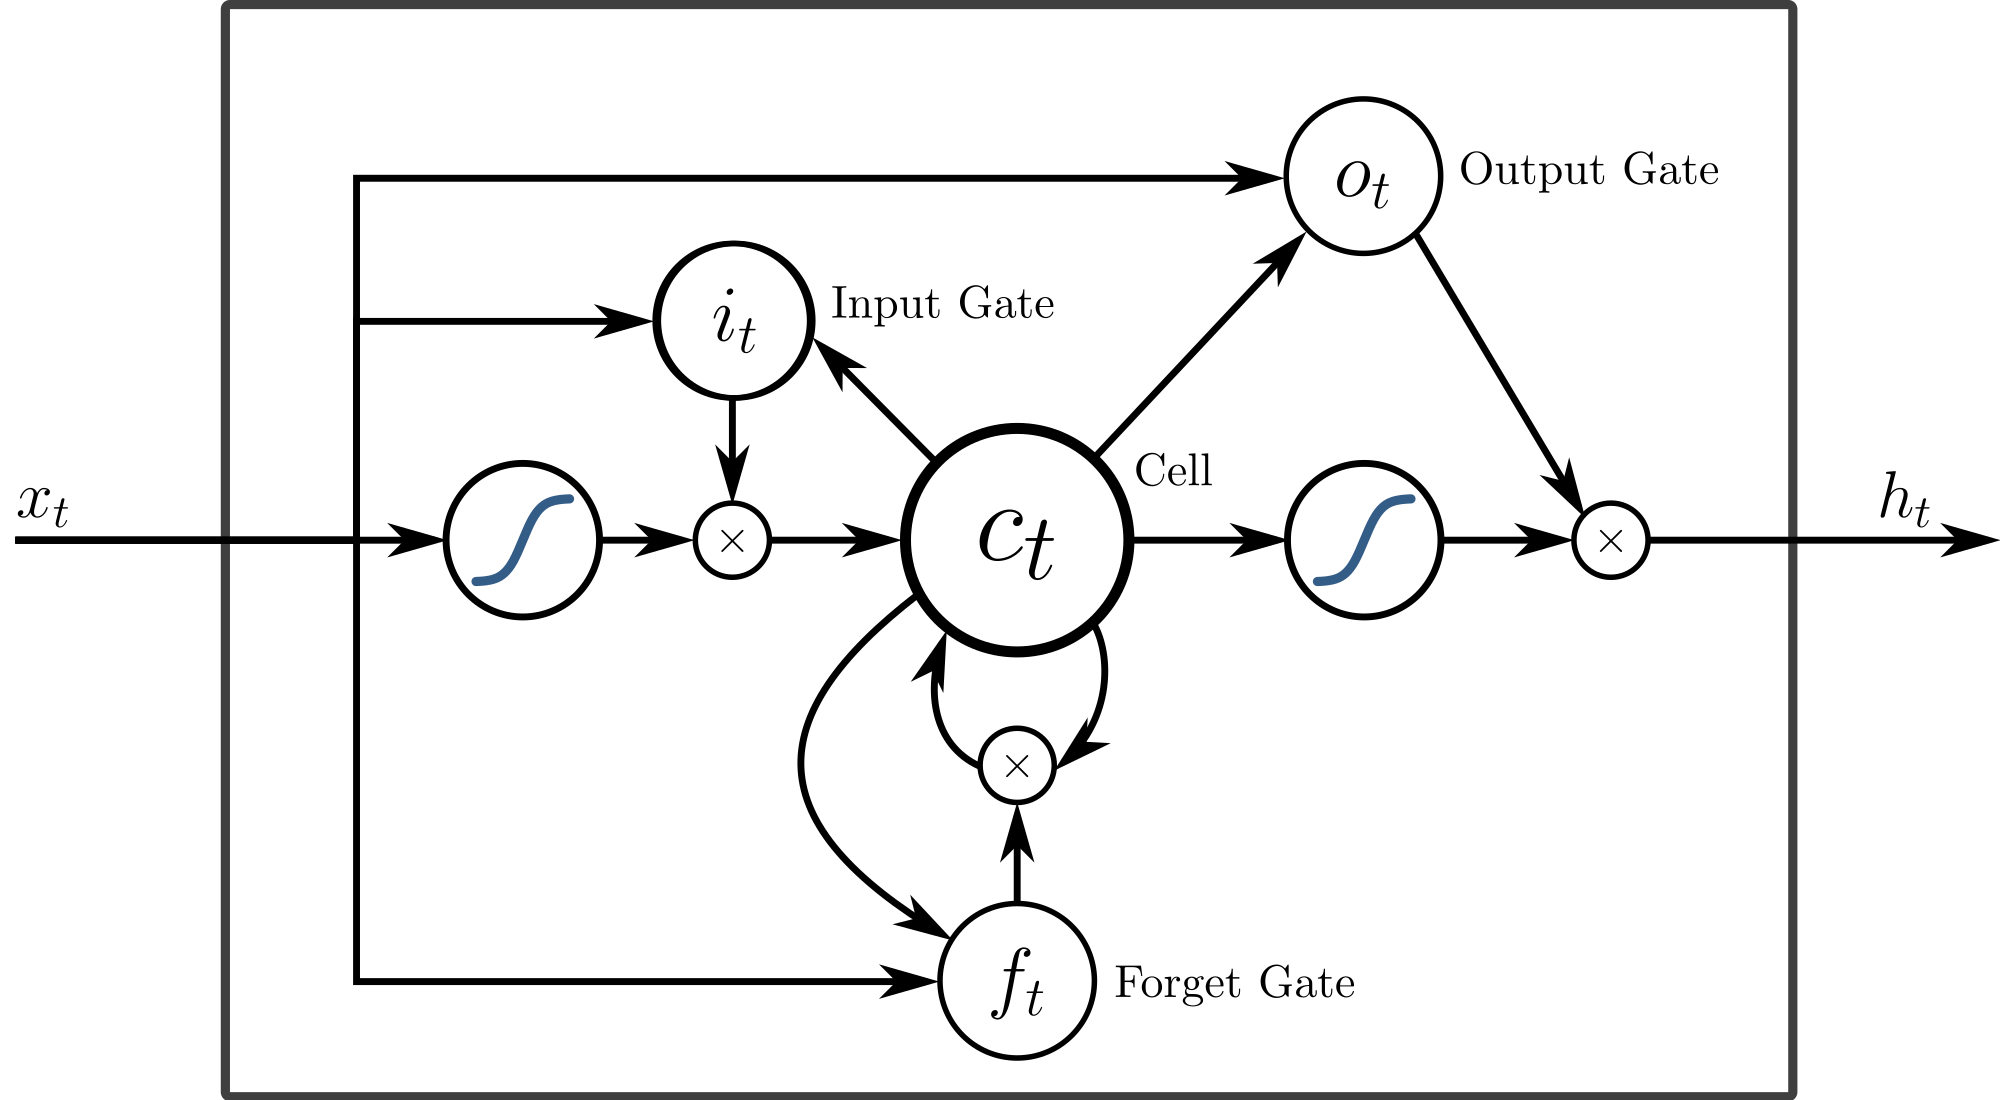
\includegraphics[scale=0.12]{img/lstm}
	\caption[]{Atminties mazgo pavyzdys\footnotemark}
	\label{img:lstm}
\end{figure}
\footnotetext{\url{https://upload.wikimedia.org/wikipedia/commons/5/53/Peephole_Long_Short-Term_Memory.svg}}

Toliau pateikiamos \textit{Tensorflow} LSTM variacijos tinklo gavimui:
\begin{itemize}
	\item \textbf{Paprastas tinklas}
        \begin{itemize}
        		\item Du sluoksniai
	        	\item Pirmajame - atsisakymo lygis 0,8
        		\item 128 - sluoksnių vienetų skaičius
        \end{itemize}

	\item \textbf{Gilus tinklas}
	\begin{itemize}
		\item Trys sluoksniai
		\item Atsisakymo lygis 0,2 visuose lygiuose
		\item 64 - sluoksnių vienetų skaičius
	\end{itemize}

	\item \textbf{Platus tinklas}
	\begin{itemize}
		\item Vienas sluoksnis
		\item Atsisakymo lygis 0,2
		\item 256 - sluoksnių vienetų skaičius	
	\end{itemize}

	\item \textbf{Platesnis tinklas}
	\begin{itemize}
		\item Vienas sluoksnis
		\item Atsisakymo lygis 0,2
		\item 512 - sluoksnių vienetų skaičius
	\end{itemize}
\end{itemize}


\subsubsubsection{GRU}
2014 metais Cho pristatė GRU modelį, kuris, buvo manyta, galės išspręsti nykstančiųjų gradientų problemą \cite{DBLP:journals/corr/ChoMGBSB14}. Šis modelis yra panašus į LSTM ir abu modeliai dažnai duoda labai panašius rezultatus.

\textbf{GRU} – uždaromas pasikartojantis vienetas (\textit{angl. gated recurrent unit}) - RNT architektūra, kuri sugeba atsimintį informaciją ilgesniam laiko tarpui. 

Kaip ir LSTM taip ir GRU naudojasi vartais. Šiuo atveju yra dviejų tipų vartai:
\begin{itemize}
	\item \textbf{Atnaujinimo vartai} (\textit{angl. update gate}) - juose apdorojama nauja įeiga sudauginta su savo svoriu ir praėjusio laiko momento paslėptoji būsena su savo svoriu. Šie vartai nusprendžia, kiek aktuali praeituose laiko momentuose turima informacija ateityje;
	\item \textbf{Atstatymo vartai} (\textit{angl. reset gate}) - šie vartai savo veiksmu niekuo nesiskiria nuo atnaujinimo vartų, tačiau jie skirti tam, kad nustatytų, kurių kitų laiko momentų informacijos verta atsisakyti.
\end{itemize}


\begin{figure}[H]
	\centering
	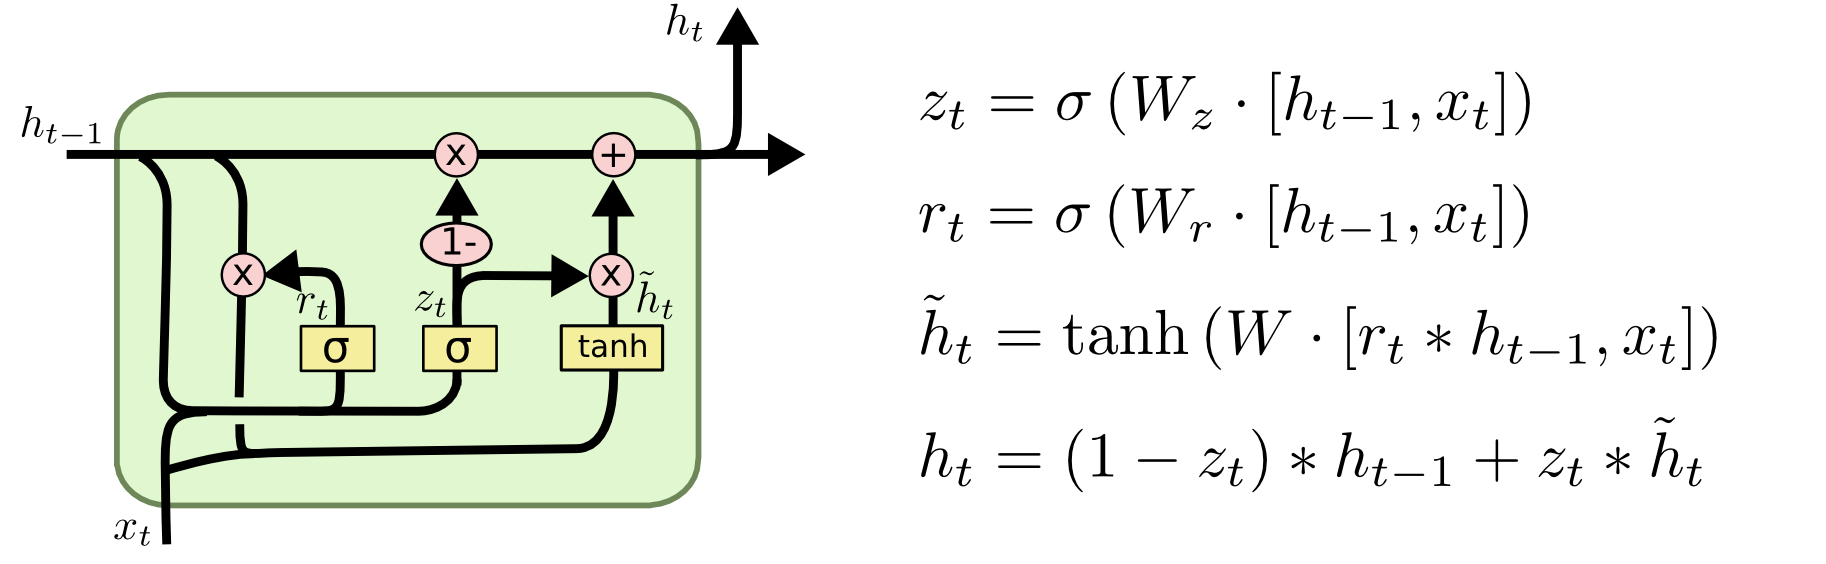
\includegraphics[scale=0.5, trim={0 0 12.9cm 0}, clip]{img/gru}
	\caption[]{GRU mazgo pavyzdys\footnotemark}
	\label{img:gru}
\end{figure}
\footnotetext{\url{https://qph.ec.quoracdn.net/main-qimg-d4725497028c5a60241e1524c32f60de.webp}}

\subsubsubsection{LSTM ir GRU skirtumai}

LSTM ir GRU skiriasi tik skirtingais skaičiavimais neuronuose. Skiriasi vartų skaičius ir juose atliekami skaičiavimai. Tačiau rezultatas tarp LSTM ir GRU yra minimalus. Dažnai šie du modeliai grąžina arba labai panašius arba netgi identiškus rezultatus ir abu puikiai sprendžia nykstančiųjų gradientų problemą. Abu apdoroja praeituose laiko momentuose sukauptą informaciją, sprendžia, ką reikėtų pasilikti, ko reikėtų atsisakyti, priimami sprendimai remiantis prieš daugiau nei vieną laiko surinkta informacija.

\subsection{Apjungiamieji tinklų modeliai}

\textbf{Apjungiamieji tinklų modeliai} - modeliai, kuriuose yra apjungiami konvoliuciniai ir rekurentiniai neuroniniai tinklai. Pagal RNT specifikacijas to daryti neturėtų būti prasmės, tačiau pagal dabartines KNT ir RNT galimybes, KNT kur kas geriau atpažįsta tam tikras pasikartojančias savybes, o RNT - jų kitimą laike. Todėl tokie apjungiamieji tinklų modeliai dažniausiai naudojami atpažįstant šnekamąją kalbą. Taip pat tokie modeliai puikiausiai tinka apjungiant įeigos sekas ir išvedant statines išeigas. 

Yra du tipai apjungiamųjų tinklų modelių:
\begin{itemize}
	\item Viena įeiga - daug išeigų. Tokiu būdu iš vieno kadro RNT sugeba aprašyti kadrą pateikiant ne vieną tame kadre matomą objektą. Pavyzdžiui, pateikiant jūros su laivu vaizdą galima gauti aprašymą, kad matomas laivas, kuris plaukia jūra.
	\item Daug įeigų - viena išeiga. Tokiu būdu iš kadrų sekos RNT sugeba generuoti vieną išeigą. Kitaip tariant duodant, pavyzdžiui, apdorojant video srautą, bus gaunama konkrečios klasės išeiga.
\end{itemize}

Galima pastebėti, kad būtent šiuo atveju, modelis, kuris apdoros video srautą ir nuspręs, kurios klasės išeiga bus gaunama yra labai naudingas. Yra žinoma, kad netgi gerai apmokius sistemą KNT ji iš kadro gali nuspręsti koks veiksmas atliekamas ar kokiai klasei yra priskiriamas kadras. Šiuo atveju norint apmokyti sistemą atpažinti gestų kalbą galima pasinaudoti KNT skirstyti gestus pakadriui ir tuomet juos apjungus RNT modeliu galima išvesti vieną bendrą klasę, kuri ir bus bendra viso vaizdo srauto klasė.

\section{Eksperimentinė dalis}

Šioje dalyje bus aprašomi visi atlikti eksperimentai ir juose gauti rezultatai.

\subsection{Panašūs darbai}
Dar prieš metus, sistemų, kurios atpažintų gestų kalbą konvoliucinių ar rekurentinių tinklų pagalba, beveik nebuvo. 2017 metais Harish Chandra Thuwal ir Adhyan Srivastava iš Jamia Millia Islamia universiteto Naujajame Delyje sukūrė konvoliucinių ir rekurentinių neuroninių tinklų modeliais paremtą sistemą, kuri sugeba atpažinti gestų kalbą iš video srauto. Šiame darbe jie vaizdo įrašą verčia į kadrų seką ir apmoko konvoliucinį tinklą. Vėliau iš šių duomenų apmoko rekurentinį neuroninį tinklą. Svarbu paminėti, kad šie du studentai pasinaudojo argentiniečių gestų kalbos duomenų rinkiniu, kuriame ant kiekvienos rankos žmonės, kurie rodė gestus, buvo užsidėję skirtingų spalvų pirštines. Taip jie iš vaizdo įrašo kadrų ištrindavo visą foną ir palikdavo tik rankas, taip apmokydami sistemą be papildomų trikdžių (\textit{angl. noise}).

\subsection{Argentiniečių gestų kalbos atpažinimas}

Buvo pasirinkta apmokyti jau esamą Harish Chandra Thuwal ir Adhyan Srivastava sukurtą modelį, jį tobulinant.

\subsubsection{Sistemos savybės}
\begin{itemize}
	\item KNT - Inception v3 modelis
	\item RNT - LSTM architektūra
\end{itemize}

\subsubsection{Bandymai}
\begin{table}[H]\footnotesize
	\centering
	\caption{Argentiniečių gestų kalbos bandymai su 3 klasėmis}
	{\begin{tabular}{| c | c | c | c | c | c | c |} \hline
		\thead{Bandymo\\Nr.} & \thead{Klasių\\skaičius} & \thead{Apmokymo\\tikslumas} & \thead{Epochų\\skaičius} & \thead{Tikslumas} & \thead{Praradimas} & \thead{Testavimas}  \\
		\hline
		1. & 3 & 100\% & 10 & 81.27\% & 0.6431 & 85.32\% \\
		\hline
		2. & 3 & 99.99\% & 100 & 89.27\% & 0.4422 & 93.33\% \\
		\hline
	\end{tabular}}
	\label{tab:asl-bandymai1}
\end{table}

Pats pirmasis bandymas buvo atliktas su trimis klasėmis, apmokant sistemą ir skaidant vaizdo įrašo kadrus kaip paveikslėlius. Kiekvienam iš jų buvo nuimamas fonas (\textit{angl. background}) ir paliekamos tik rankų plaštakos, todėl buvo toks didelis apmokymo tikslumas.

Antruoju bandymu buvo atsisakyta nuimti foną ir palikti kadrus tokius, kokie yra. Dėl padidinto epochų skaičiaus rezultatai gauti geresni nei pirmuoju bandymu.

\begin{table}[H]\footnotesize
	\centering
	\caption{Argentiniečių gestų kalbos bandymai su 25 klasėmis}
	{\begin{tabular}{| c | c | c | c | c | c | c |} \hline
		\thead{Bandymo\\Nr.} & \thead{Klasių\\skaičius} & \thead{Apmokymo\\tikslumas} & \thead{Epochų\\skaičius} & \thead{RNT\\apmokymo\\tipas} & \thead{Tikslumas} & \thead{Praradimas}  \\
		\hline
		1. & 25 & 91.90\% & 100 & Platus & 91.99\% & 0.6839 \\
		\hline
		2. & 25 & 91.90\% & 100 & Platesnis & 91.95\% & 0.6255 \\
		\hline
		3. & 25 & 91.90\% & 100 & Gilus & 16.55\% & 2.0566 \\
		\hline
		4. & 25 & 91.90\% & 10 & Paprastas & 97.61\% & 0.2814 \\
		\hline
		5. & 25 & 91.90\% & 100 & Paprastas & 92.66\% & 0.5539 \\
		\hline
	\end{tabular}}
	\label{tab:asl-bandymai2}
\end{table}

\ref{tab:asl-bandymai2} lentelėje pateikiami dar 5 bandymai atlikti su argentiniečių gestų kalba. Šiuo atveju sistemos KNT modelis buvo apmokytas vieną kartą, o toliau buvo keičiami RNT apmokymo būdai. Šie būdai buvo paremti LSTM modeliu. Galima pastebėti, kad giliuoju (\textit{angl. deep}) būdu rezultatai buvo prasčiausi. 

\subsection{Lietuvių gestų kalbos atpažinimas}

Nėra jokios mokslinės literatūros, kurioje būtų aprašyti lietuvių gestų kalbos atpažinimui skirti modeliai, kurie remiasi konvoliuciniais ar rekurentiniais neuroniniais tinklais. Šie bandymai, manoma, kad yra pirmieji naudojantis rekurentiniais neuroniniais tinklais atpažinti LGK. Konvoliucinių neuroninių tinklų pagalba tokį darbą dariau prieš metus, skirtą atpažinti statinę gestų kalbos abėcėlę pasinaudojant Inception v3 modeliu.

Šių eksperimentų tikslas - išbandyti galimybes atpažinti gestų kalbą, nes lietuvių gestų kalbos atpažinimas iš video srauto galėtų palengvinti ne tik gestų kalbos nesuprantantiesiems bendrauti su gestakalbiais, bet ir, pavyzdžiui, turėti galimybę versti žodinę kalbą į gestų kalbą. 

Toliau pateikiamas visas darbas padarytas su lietuvių gestų kalbos atpažinimu, duomenų rinkimu ir gautais rezultatais.

\subsubsection{Duomenų paruošimas}
Oficialiame lietuvių gestų kalbos žodyne, kurį pristato \textbf{neįgaliųjų reikalų departamentas prie socialinės apsaugos ir darbo ministerijos}, pateikiama apie 9000 gestų. Žodynas rengiamas nuo 2004 metų kurčiųjų ir girdinčiųjų komandos. Šiame žodyne gestus galima rasti pagal žodį, gesto formą ar temą. Taip pat galima pasirinkti ar gesto ieškoti kaip atitinkamo žodžio ar naudojimo pavyzdžiuose. Susiradus tinkamą žodį yra aprašomos tokios specifikos kaip plaštakos forma, lūpų judesys, žodžio ar sakinio reikšmė. 

Naudojantis šiuo žodynu iškyla viena pagrindinė problema - kiekvienas gestas turi tik po vieną video įrašą atitinkantį tą žodį. Toks kiekis duomenų yra per mažas, norint apmokyti sistemą RNT būdu. Galima iš sakinių, kuriuose yra žodžio naudojimo pavyzdžiai, taip pat išskirti gestus, atitinkančius norimą gestą. Tačiau tai padidintų kiekvienos klasės duomenų kiekį iki daugiausiai 5 vaizdo įrašų. Net ir toks duomenų kiekis yra per mažas.

Nuspręsta duomenis susikurti. Teko pramokti lietuvių gestų kalbos gestus. Įsigilinti į gestų kalbos specifiką. Pirmiesiems bandymams buvo nufilmuota 3 skirtingų žodžių klasių gestai po 50 vaizdo įrašų kiekvienam iš jų, kas yra tapatu 150 video įrašų. Filmuota buvo mobiliuoju telefonu rodančiąjam atsistojus prie gelsvos sienos. Filmuoti buvo du skirtingi asmenys, kurių kiekvienas atliko po 25 vaizdo įrašus kiekvienai klasei. Buvo pasirinkta pirmiesiems bandymams pasinaudoti „labas“, „mano“, „vardas“ žodžių klasėmis. Kiekvienas vaizdo įrašas truko ne ilgiau nei 3 sekundes.

Vėliau buvo nufilmuotos dar 10 skirtingų gestų klasių. Šiuo atveju buvo nufilmuota nebe 50, o 20 kiekvieno gesto įrašų. Kaip ir pirmuoju filmavimu, taip ir šiuo, buvo filmuojami du skirtingi asmenys. Galiausiai buvo nufilmuota dar 12 papildomų klasių, todėl bendras duomenų rinkinys buvo sudarytas iš 25 skirtingų lietuvių gestų kalbos gestų klasių.

\textbf{Rezultatas} – duomenų bazė sudaryta iš 25 skirtingų LGK klasių po 20-50 video įrašų. Kiekvieno video trukmė ne ilgesnė nei 4 sekundės, kas tapatu ne daugiau nei 120 kadrų\footnote{1 sekundė = 30 kadrų} kiekvienam įrašui. \ref {tab:lgk-duomenys} lentelėje pateikiamos visos nufilmuotos klasės ir vaizdo įrašų kiekis paruoštas kiekvienam gestui.

\begin{table}[H]\footnotesize
	\centering
	\caption{LGK paruošti duomenys}
	{\begin{tabular}{| c | c | c || c | c | c || c | c | c |}
		\hline
		\thead{Nr.} & \thead{Klasė} & \thead{Kiekis}  & \thead{Nr.} & \thead{Klasė} & \thead{Kiekis} & \thead{Nr.} & \thead{Klasė} & \thead{Kiekis}  \\
		\hline
		1. & labas & 50 & 10. & radijas & 20 & 19. & juodas & 20 \\
		\hline
		2. & mano & 50 & 11. & šuo & 20 & 20. & lėktuvas & 20 \\
		\hline
		3. & vardas & 50 & 12. & katė & 20 & 21. & autobusas & 20 \\
		\hline
		4. & jėga & 20 & 13. & višta & 20 & 22. & limonadas & 20 \\
		\hline
		5. & nuoširdus & 20 & 14. & laikrodis & 20 & 23. & kava & 20 \\
		\hline
		6. & nuostabus & 20 & 15. & kapinės & 20 &  24. & pietūs & 20 \\
		\hline
		7. & mama & 20 & 16. & laimėti & 20 & 25. & žaizda & 20 \\
		\hline
		8. & tėtis & 20 & 17. & vestuvės & 20 \\
		\cline{1-6}
		9. & kompiuteris & 20 & 18. & gydytojas & 20 \\
		\cline{1-6}
	\end{tabular}}
	\label{tab:lgk-duomenys}
\end{table}


\subsubsection{Modelio apmokymas}

Modelį buvo nuspręsta apmokyti pasinaudojant Harish Chandra Thuwal ir Adhyan Srivastava jau sukurtu modeliu, jau atliktus jam patobulinimus išbandant argentiniečių gestų kalbos atpažinimą. Vienas iš svarbiausių pakeitimų - nenutrinti fono kadruose. Taip pat pakeistas epochų skaičius, RNT LSTM tinklo apmokymo tipas, perdarytas testavimo mechanizmas.

Visų pirma buvo apmokyta sistema su trimis klasėmis „labas“, „mano“ ir „vardas“, turinčiomis po 50 vaizdo įrašų (\textit{žr. \ref{tab:lgk-duomenys} lentelė}). Šie gestai visi atliekami dešiniąja ranka, todėl tai sistemai, buvo manyta, turėtų šiek tiek palengvinti darbą su duomenimis.

Pirmiausiai kiekvienas vaizdo įrašas buvo išskaidomas į kadrus. Dažniausiai gesto vaizdo įrašas truko apie 2 sekundes, bet ne ilgiau 3 sekundžių. Tai reiškia, kad filmuojant mobiliuoju įrenginiu pasirinkus 30 kadrų per sekundę būdą, kiekvienas gestas turėdavo apie 60 kadrų, daugiausiai 90 kadrų. Buvo nuspręsta padaryti vienodus kiekius kadrų kiekvienam gestui. Tokiu atveju kadrų kiekis buvo pakeltas iki 120 kadrų kiekvienam vaizdo įrašui, kas lygu 4 sekundėms vaizdo įrašo. Kadangi visi įrašai skyrėsi savo ilgiu buvo nuspręsta, jei vaizdo įrašas per trumpas, paskutinį kadrą kartoti tiek kartų, kad visi įrašai turėtų vienodą kiekį kadrų. 

Buvo priimti tokie sprendimai, remiantis jau turimu argentiniečių gestų kalbos patobulintu apjungtu neuroniniu tinklu:
\begin{enumerate}
	\item Vaizdo įrašą skaidyti į 120 kadrų (vietoje 200 turimame mokymo mechanizme). Jei įrašas per trumpas - paskutinį kadrą kartoti $n$ kartų, kol bus 120 kadrų;
	\item Konvoliucinį neuroninį tinklą apmokyti Inception v3 modeliu (\textit{žr. \ref{appendix:inception_v3} priede});
	\item RNT apmokyti pasirinkus paprastą modelį, kuris naudojasi LSTM architektūra;
	\item Mokymo - testavimo aibę skaidyti į 80\% mokymui ir 20\% testavimui, todėl mokymui buvo skirta 40 vaizdo įrašų, o testavimui - 10.
\end{enumerate}

\subsubsubsection{3 klasių apmokymas}
\underline{Duomenys:}
\begin{itemize}
	\item 3 klasės - „labas“, „mano“, „vardas“;
	\item 40 vaizdo įrašai kiekvienai klasei. Viso - 120;
	\item 10 vaizdo įrašų kiekvienos klasės testavimui. 
\end{itemize}

\bigbreak
\textbf{Pirmasis bandymas}

\underline{Rezultatai:}
\begin{itemize}
	\item KNT: galutinis tikslumas (\textit{angl. final test accuracy}) - 98.9\%;
	\item Buvo atlikti spėjimai su KNT, kuris teisingai atspėjo 14307 iš 14400 kadrų (tikslumas - 99.35\%);
	\item RNT: Tikslumas 86.93\% ir 0.5081 praradimas;
	\item Mokymosi grafikai pateikiami \ref{appendix:3kl} priede.
\end{itemize}

\bigbreak
\textbf{Antrasis bandymas}

\underline{Pakeitimai:}

Nuspręsta, jei vaizdo įrašas yra mažesnis nei 120 kadrų, kartoti kadrus nebe gale, kaip buvo ligi tol, bet juos pakartoti viduryje. Šio metodo išbandymui buvo pasinaudota pakartoti kadrus daugiausiai du kartus. Pavyzdžiui, jei įrašas yra 60 kadrų, tai kiekvieną kadrą pakartoti po du kartus. Jei įrašas 90 kadrų, tai kartoti 45-75 kadrus po du kartus. Tačiau buvo nuspręsta, kad jei vaizdo įrašas trumpesnis nei 60 kadrų, kartoti likusius kadrus $60-n$, kur $n$ - kadrų skaičius, pasinaudojant paskutiniu kadru.

\underline{Rezultatai:}
\begin{itemize}
	\item KNT: galutinis tikslumas - 99.0\%;
	\item Buvo atlikti spėjimai su KNT, kuris teisingai atspėjo 14270 iš 14400 kadrų (tikslumas - 99.10\%);
	\item RNT: Tikslumas 87.5\% ir 0.4995 praradimas;
	\item Mokymosi grafikai pateikiami \ref{appendix:3kl} priede.
\end{itemize}

\bigbreak
\textbf{Trečiasis bandymas}

\underline{Pakeitimai:}

Nuspręsta patobulinti antruoju bandymu padarytą pakeitimą. Padaryta, kad jei vaizdo įrašas yra trumpesnis nei 60 kadrų, tada kartoti kadrus po 3 kartus. Jei ilgesnis nei 60 ir trumpesnis nei 120 - 2 kartus. Kadangi trumpesnių vaizdo įrašų nei 40 kadrų nebuvo, tai tikslo kartoti kadrus po 4 kartus taip pat nebuvo.

\underline{Rezultatai:}
\begin{itemize}
	\item KNT: galutinis tikslumas - 99.1\%;
	\item Buvo atlikti spėjimai su KNT, kuris teisingai atspėjo 14307 iš 14400 kadrų (tikslumas - 99.35\%);
	\item RNT: Tikslumas 88.33\% ir 0.4832 praradimas;
	\item Mokymosi grafikai pateikiami \ref{appendix:3kl} priede.
\end{itemize}

\bigbreak
\textbf{Apibendrinimas}

Šiais trimis bandymais naudojantis trimis skirtingomis LGK klasėmis buvo pastebėta, kad geresni rezultatai gaunami tuomet, kai kartojamas gestas yra viduryje, kuomet ir yra svarbiausia jį pastebėti ir atpažinti. Toks sprendimas buvo priimtas dėl KNT apsimokymo galimybių ir bendrų savybių išskyrimo. Kartojimas tose vietose, kuriose labiausiai pasireiškia gesto savybės ir jo atskyrimas nuo kitų klasių, yra geresnis sprendimas apmokant KNT, nei kartojimas pačiame vaizdo įrašo gale, pasinaudojant paskutiniu kadru, nes tuomet rodantysis stovi nuleidęs rankas ar pozicijoje, kurioje didžiojoje klasių dalyje yra pradedami ir pabaigiami gestai.

Pastebėta, kad rezultatai ypatingai nesiskyrė, bet gauti geriausi rezultatai, nors ir minimalūs, paskutiniu bandymu. Nuspręsta naudotis šiuo (trečiuoju bandymu) susikurtu metodu, vykdant tolimesnius apmokymus pasinaudojant daugiau klasių.

\subsubsubsection{10 klasių apmokymas}

Antruoju apmokymu buvo pasirinktos 10 klasių (4-13 klasės (\textit{žr. \ref{tab:lgk-duomenys} lentelę})). Kadangi buvo nufilmuota po 20 kiekvienos iš šių klasių vaizdo įrašų, tai buvo nuspręsta pasinaudojus \textit{OpenCV} bibliotekos savybėmis, skaidant vaizdo įrašus į kadrus praplėsti vaizdo įrašų aibę iki 50. 

Kiekvieną vaizdo įrašą skaidant į gestus, jei gestas per trumpas, gesto vaizdo įrašo centrinė dalis kartojama 2-3 kartus (\textit{plačiau - 3.3.2.1. 3 klasių apmokymas. Trečiasis bandymas}). 

Prieš skaidant vaizdo įrašus į kadrus, iš eilės, jei vaizdo įrašų kiekis klasėje yra mažesnis nei 50, kiekvienas vaizdo įrašas yra pakartojamas antrąjį kartą. Jei mažesnis nei 25 - vaizdo įrašas pakartojamas trečiąjį kartą. Taip daroma tol, kol bendras skaičius vaizdo įrašų pasiekia 50. Tačiau kiekvienam vaizdo įrašo pakartojimui yra pritaikomos modifikacijos. Vaizdo įrašo kadrai yra ištempiami ir suspaudžiami pasinaudojus atsitiktinėmis transformacijomis.

\begin{figure}[H]
	\centering
	\begin{minipage}{.27\textwidth}
		\centering
		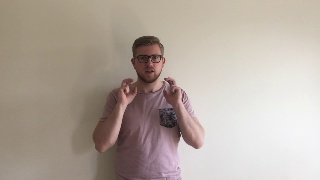
\includegraphics[width=.8\linewidth]{img/other/org}
		\caption[a]{Orginalus vaizdo įrašo kadras}
		\label{img:lgk10-1}
	\end{minipage}
	\qquad
	\begin{minipage}{.27\textwidth}
		\centering
		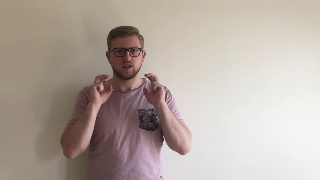
\includegraphics[width=.8\linewidth]{img/other/m1}
		\caption[b]{Modifikuotas 12 pav. kadras}
		\label{img:lgk10-2}
	\end{minipage}%
	\qquad
	\begin{minipage}{.27\textwidth}
		\centering
		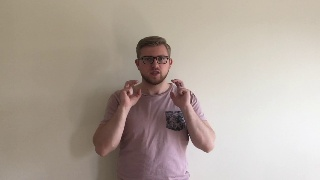
\includegraphics[width=.8\linewidth]{img/other/m2}
		\caption[c]{Modifikuotas 12 pav. kadras}
		\label{img:lgk10-3}
	\end{minipage}
\end{figure}

Kiekvienas kadras vaizdo įraše buvo 1280 $\times$ 720 taškų. Anksčiau kiekvienas kadras ir būdavo saugomas tokiu pačiu dydžiu. Nuspręsta sumažinti kadrus iki 320 $\times$ 180. Tai padidino greitį ir labai sumažino užimamos vietos kiekį, kadangi taškų kiekis kadre buvo sumažintas 16 kartų.

Taip pat, šiame žingsnyje buvo pritaikytas automatinis LGK klasių vaizdo įrašų išskaidymas į mokymo-testavimo aibes. Generuojant naujus vaizdo įrašus paskutiniai 20\% vaizdo klasės įrašų buvo perkeliami į testavimo aplanką (\textit{angl. folder}).

Šio apmokymo metu visi bandymai buvo atlikti konvoliucinį neuroninį tinklą apmokius vieną kartą.

Buvo nuspręsta pasinaudoti giliuoju RNT tinklu vietoje paprasto.

\underline{Duomenys:}

\begin{itemize}
	\item 10 klasių;
	\item 20 vaizdo įrašų kiekvienai klasei;
	\item Sugeneruota 40 vaizdo įrašų kiekvienai klasei;
	\item Sugeneruota 10 vaizdo įrašų kiekvienos klasės testavimui.
\end{itemize}

\bigbreak
\textbf{Pirmasis bandymas}

\underline{Rezultatai:}
\begin{itemize}
	\item KNT: galutinis tikslumas - 96.3\%;
	\item RNT: Tikslumas 93.58\% ir 0.3727 praradimas;
	\item Mokymosi grafikai pateikiami \ref{appendix:10kl} priede.
\end{itemize}

\bigbreak
\textbf{Antrasis bandymas}

\underline{Pakeitimai:}

Nuspręsta padidinti RNT epochų skaičių nuo 50 iki 100 ir pakeisti iš gilaus tiklo į paprastą tinklą.

\underline{Rezultatai:}
\begin{itemize}
	\item KNT: galutinis tikslumas - 96.3\%;
	\item RNT: Tikslumas 45.61\% ir 1.419 praradimas;
	\item Mokymosi grafikai pateikiami \ref{appendix:10kl} priede.
\end{itemize}


\bigbreak
\textbf{Trečiasis bandymas}

\underline{Pakeitimai:}

Pastebėjus, kad gauti labai prasti rezultatai antruoju bandymu, buvo nuspręsta vėl pasinaudoti giliu tinklu, bet palikti 100 epochų skaičių.

\underline{Rezultatai:}
\begin{itemize}
	\item KNT: galutinis tikslumas - 96.3\%;
	\item RNT: Tikslumas 94.28\% ir 0.3563 praradimas;
	\item Mokymosi grafikai pateikiami \ref{appendix:10kl} priede.
\end{itemize}

\bigbreak
\textbf{Apibendrinimas}

Pastebėta, kad didinant epochų skaičių (pirmas ir trečias bandymai) galutinis RNT tikslumas kinta, bet nėra didelis. Šio apmokymo pabaigoje buvo nuspręsta, kad geriau palikti 50 epochų skaičių vietoje 100, kadangi rezultatas beveik nekinta, o laiko užima 2 kartus daugiau. Taip pat pastebėta, kad 3 klasių apmokyme paprastas RNT LSTM tinklas buvo puikus sprendimas, duodantis po 10 epochų labai aukštus rezultatus, tačiau padidinus klasių skaičių nuo 3 iki 10, paprastas tinklas grąžina prastus rezultatus. To pasekoje buvo nuspręsta geriau naudoti gilųjį tinklą vietoj paprastojo tęsiant bandymus.

\subsubsubsection{25 klasių apmokymas}

Trečiojo apmokymo metu buvo pasinaudota visomis duomenų paruošimo stadijoje pasiruoštomis klasėmis (\textit{žr. \ref{tab:lgk-duomenys} lentelę}).  Kiekviena klasė turėjo 20 (22 klasės) arba 50 (3 klasės) vaizdo įrašų. Naudojantis antruoju apmokymo metu susikurtu duomenų dauginimo mechanizmu, kuris leido 20 vaizdo įrašų duomenis paversti į 50. Taip pat automatiškai buvo išskaidoma mokymo-testavimo aibė. Reikėtų pastebėti ir tai, kad buvo pasinaudota ir 10 klasių apmokymo stadijoje sumažintu kadrų taškų skaičiumi. Tai vėlgi sutaupė labai daug užimamos vietos, bet neturėjo jokios įtakos tikslumui.

\underline{Duomenys:}

\begin{itemize}
	\item 25 klasės;
	\item 20-50 vaizdo įrašų kiekvienai klasei;
	\item Sugeneruota 40 vaizdo įrašų kiekvienai klasei;
	\item Sugeneruota 10 vaizdo įrašų kiekvienos klasės testavimui.
\end{itemize}

\underline{Rezultatai:}
\begin{itemize}
	\item KNT: galutinis tikslumas (\textit{angl. final test accuracy}) - 89.1\%;
	\item RNT: Tikslumas 92.89\% ir 0.4361 praradimas;
	\item Mokymosi grafikai pateikiami \ref{appendix:25kl} priede.
\end{itemize}

\subsubsubsection{Apibendrinimas}
Toliau, \ref{tab:lgk-bandymai} lentelėje pateikiami visų trijų apmokymų su lietuvių gestų kalba geriausi gautų modelių rezultatai.

\begin{table}[H]\footnotesize
	\centering
	\caption{Lietuvių gestų kalbos apmokymų rezultatai}
	{\begin{tabular}{| c | c | c | c | c | c | c |}
		\cline{4-7}
		\multicolumn{3}{ c |}{} & 
		\multicolumn{1}{ c |}{\thead{KNT}} &
		\multicolumn{3}{ c |}{\thead{RNT}} \\
		\hline
		\thead{Bandymo\\Nr.} & \thead{Klasių\\skaičius} & \thead{Vaizdo\\įrašų\\skaičius}  & \thead{Tikslumas} & \thead{Epochų\\skaičius}& \thead{Tikslumas} & \thead{Praradimas}  \\
		\hline
		1. & 3 & 120 & 99.1\% & 100 & 88.33\% & 0.4832 \\
		\hline
		2. & 10 & 400 & 96.3\% & 100 & 94.28\% & 0.3563 \\
		\hline
		3. & 25 & 1000 & 89.1\% & 50 & 92.89\% & 0.4361 \\
		\hline
	\end{tabular}}
	\label{tab:lgk-bandymai}
\end{table}

Galima pastebėti, kad nėra didelio KNT ir RNT tikslumų ir praradimų skirtumo tarp modelių juos apmokius. Pastebėta, kad epochų skaičius apmokant RNT - 50 ar 100 - neturi didelės įtakos bendro modelio tikslumo gerinimui. Taip pat verta pastebėti, kad klasių skaičius nedarė didelės įtakos KNT ir RNT tikslumams. 

Matomas tikslumo mažėjimas KNT modelio didėjant klasių skaičiui. Šis tikslumas mažėja, manoma, todėl, kad didesnis klasių skaičius ir tarpusavyje tarp klasių esantys bendri panašumai sunkina gesto atpažinimą iš kadro. Juolab svarbu ir tai, kad KNT mokosi iš kiekvieno kadro atskirai ir jų kitimas laike turi įtakos bendram rezultatui.

Kintant klasių skaičiui didėja RNT modelio tikslumas. Manoma, taip yra todėl, kad didesnis bendras duomenų kiekis leidžia geriau apsimokyti sistemai, kadangi apmokant 25 klasių modelį buvo sukurta daugiau nei 120 tūkstančių kadrų, iš kurių mokėsi modelis (palyginimui - 3 klasių modeliui buvo sukurti virš 14 tūkstančių kadrų). 

Lyginant rezultatus, manoma, kad didesniam nei 88\% daug įtakos tikslumui turėjo ir gerai paruošta LGK duomenų bazė. Toks bazės paruošimas palengvina apsimokymo procesą, pagerina rezultatus. Daug triukšmo ir netinkamų duomenų turintys rinkiniai, turėtų daug įtakos blogesniems rezultatams.

Reikėtų labiau įsigilinti į rezultatų priklausomybę nuo klasių ir apmokymo nustatymų. Reikėtų išbandyti RNT LSTM platų, platesnį būdus su geriausiais modeliais ir stebėti bendrus pasikeitimus. Taip pat reikėtų išbandyti didesnę duomenų augmentaciją, mokymui skirtą duomenų bazę praplėsti, išbandyti su daugiau klasių ir mokymo rinkinį paruošti iš daugiau skirtingų rodančiųjų duomenų bei daugiau trikdžių ir triukšmo turinčioje aplinkoje, pavyzdžiui, miške, prie spalvotų sienų ar kitur.

\subsubsection{Modelio testavimas}

Turimi visi trys modeliai buvo ištestuoti su 20\% visų duomenų. Kiekvienas testavimo vaizdo įrašas buvo skaidomas į kadrus kaip ir apmokymo metu. Tačiau sistema KNT pagalba tik spėliojo pagal kadrus, koks tai gestas galėtų būti ir tuomet visa surinkta informacija, buvo duodama RNT galutiniam sprendimui padaryti. Toliau pateikiami visų trijų apmokymų testavimai ir jų rezultatai.

\begin{table}[H]\footnotesize
	\centering
	\caption{Lietuvių gestų kalbos modelių testavimo rezultatai}
	{\begin{tabular}{| c | c | c | c |}
		\hline
		\thead{Bandymo\\Nr.} & \thead{Nematytų\\duomenų\\kiekis} & \thead{KNT\\pasirinkimas}  & \thead{RNT\\pasirinkimas}  \\
		\hline
		1. & 30 & 83.92\% & 79.31\% \\
		\hline
		2. & 100  & 90.26\% & 87.34\% \\
		\hline
		3. & 250 & 88.17\% & 79.18\% \\
		\hline
	\end{tabular}}
	\label{tab:lgk-testavimas}
\end{table}

\ref{tab:lgk-testavimas} lentelėje pateikiami lietuvių gestų kalbos sukurtų modelių testavimo rezultatai. Duomenys (vaizdo įrašai) duoti apmokymui ir testavimui beveik nesiskyrė. Kiekvieno vaizdo įrašas buvo automatiškai išskirstomas ar tai bus skirtas testavimui ar apmokymui. 

Galima pastebėti, kad modeliai su dideliu tikslumu teisingai nusprendžia rodomo gesto klasę. Įdomu tai, kad kiekvienas modelis galutinį teisingą atsakymą atspėdavo 4 kartus iš 5. Tai rodo, kad modeliui didelės įtakos nedaro ar jis apmokytas atpažinti 3 ar 25 klases. 

25 gestų klasių testavimo metu buvo pastebėta, kad nebuvo nei vieno teisingo galutinio atsakymo testuojant „višta“ klasę. Visais atvejais modelis spėjo „tėtis“ klasę, kadangi gestai yra ganėtinai panašūs - rodomi dešine ranka, rodomuoju (2) pirštu pradedant gestą nuo smakro. Skyrėsi tai, kad „vištos“ geste 1 ir 2 pirštai imituoja vištos snapą, o „tėtis“ klasėje 2 pirštas nuo smakro pakeliamas iki kaktos. 

Geresniems ir tikslesniems testavimo rezultatams gauti reikėtų pirmiausia pabandyti ištestuoti su daugiau gestų pavyzdžių. Taip pat reikėtų išbandyti šių modelių testavimą su kitų žmonių rodomais gestais. Manoma, kad nufilmavus gestus trikdžių pilnoje aplinkoje, testavimo rezultatai būtų kur kas prastesni. 

\subsection{Duomenų rinkimo rekomendacijos}

Naudojantis jau sukaupta patirtimi ir atliktais eksperimentais aprašytais šiame darbe yra \textbf{rekomenduojama}:

\begin{itemize}
	\item Naujų lietuvių gestų kalbos klasių rinkimas ir peržiūra;
	\item Jau esamų LGK klasių pildymas;
	\item Vaizdo įrašų kiekis kiekvienoje klasėje neprivalo būti vienodas, tačiau patartina turėti bent 20 vaizdo įrašų kiekvienai klasei;
	\item Pirmiesiems apmokymams vaizdo įrašai turi būti gerai atrinkti ir be papildomų trikdžių;
	\item Vertėtų rinkti ir trikdžių (pasikeitusi aplinka, neypač tiksliai parodytas gestas ir kt.) turinčius vaizdo įrašus, tam, kad papildomai galima būtų apmokyti modelį atpažinti gestų klases įvairiose aplinkose;
	\item Patartina, kad gestus rodytų skirtingi asmenys.
\end{itemize}


\sectionnonum{Rezultatai ir išvados}

\subsectionnonumnocontent{Rezultatai}
\begin{enumerate}
	\item Išanalizuotos konvoliucinių ir rekurentinių neuroninių tinklų ypatybės;
	\item Suformuluota RNT užduotis pasinaudojant daug su vienu sąryšiu;
	\item Išanalizuotos gestų kalbos vienetų atpažinimo iš video srauto galimybės. Pastebėta, kad geriausias būdas tai daryti - pasinaudoti apjungtuoju neuroninių tinklų modeliu;
	\item Sukurta lietuvių gestų kalbos 25 skirtingų gestų duomenų bazė, susidedanti iš 22 klasių, kurių kiekviena turi po 20 vaizdo įrašų, ir 3 klasių, kurių kiekviena turi po 50 vaizdo įrašų;
	\item Sukurti trys skirtingi lietuvių gestų kalbos modeliai, kurie atpažįsta 3, 10 ir 25 skirtingas LGK klases;
	\item Sukurti trys lietuvių gestų kalbos modeliai buvo apmokyti su 80\% ir ištestuoti su 20\% visų duomenų;
	\item Geriausius rezultatus davė 10 klasių modelis (87,34\%), tačiau didesnį panaudojamumą turi 25 klasių modelis, kuris 79,18\% tikslumu prognozuodavo rodomo gesto klasę.
\end{enumerate}


\subsectionnonumnocontent{Išvados}
\begin{enumerate}
	\item Pastebėta, kad dinaminė gestų kalba ir jos mokymąsis yra sudėtingas procesas, reikalaujantis labai daug laiko ir pastangų;
	\item Išsiaiškinta, kad apjungtieji neuroniniai tinklai, kurie apjungia KNT ir RNT, gali būti plačiai pritaikomi tuose uždaviniuose, kuriuose reikalinga rasti savybes kiekviename laiko momente ir tas savybes apjungti į bendrą visumą. Taip pat išsaiškinta, kad idealiu atveju tokių apjungimų nereikėtų, tačiau šiuo metu RNT akcentuojasi labiau į kitimą laike, nei į savybių atpažinimą;
	\item Apjungtieji neuroniniai tinklai, kurie remiasi KNT ir RNT apjungtais modeliais yra labai galingas ir puikiai panaudojamas įrankis gestų kalbos atpažinime;
	\item Išsiaiškinta, kad vaizdo įrašus skaidant į kadrus ypač svarbu atkreipti dėmesį į kadro dydį, nes tai turi labai daug įtakos apsimokymo laikui ir užimamos vietos kiekiui, tačiau kadrų mažinimas beveik neturi įtakos modelio tikslumui;
	\item Nustatyta, kad klasių skaičius (3, 10 ar 25) neturi didelės įtakos apsimokymo tikslumui ir testavimo rezultatams;
	\item Gauti aukšti rezultatai rodo gerai sudarytą apmokymui skirtų duomenų rinkinį, tačiau nėra aišku, koks tikslumas gautųsi testuojant ar apmokant su realių situacijų duomenimis;
	\item Norint lietuvių gestų kalbos modelį pritaikyti realiame pasaulyje, reikia daugiau studijų šioje srityje ir apmokyti jį su kelis kartus didesniu LGK klasių kiekiu;
	\item Reikėtų kaupti lietuvių gestų kalbos gestų vaizdo įrašus, kad šiuos modelius būtų galima apmokyti atpažinti daugiau klasių. Surinkus užtektinai didelį duomenų kiekį, sistema būtų pritaikyta versti gestų kalbą į rašytinę kalbą ir atvirkščiai.
\end{enumerate}
%
%Rezultatų ir išvadų dalyje išdėstomi pagrindiniai darbo rezultatai (kažkas
%išanalizuota, kažkas sukurta, kažkas įdiegta), toliau pateikiamos išvados
%(daromi nagrinėtų problemų sprendimo metodų palyginimai, siūlomos
%rekomendacijos, akcentuojamos naujovės). Rezultatai ir išvados pateikiami
%sunumeruotų (gali būti hierarchiniai) sąrašų pavidalu. Darbo rezultatai turi
%atitikti darbo tikslą.

\printbibliography[heading=bibintoc]  % Šaltinių sąraše nurodoma panaudota
% literatūra, kitokie šaltiniai. Abėcėlės tvarka išdėstomi darbe panaudotų
% (cituotų, perfrazuotų ar bent paminėtų) mokslo leidinių, kitokių publikacijų
% bibliografiniai aprašai. Šaltinių sąrašas spausdinamas iš naujo puslapio.
% Aprašai pateikiami netransliteruoti. Šaltinių sąraše negali būti tokių
% šaltinių, kurie nebuvo paminėti tekste. Šaltinių sąraše rekomenduojame
% necituoti savo kursinio darbo, nes tai nėra oficialus literatūros šaltinis.
% Jei tokių nuorodų reikia, pateikti jas tekste.

\sectionnonum{Santrumpos}
\begin{itemize}
	\item KNT - konvoliuciniai neuroniniai tinklai
	\item LGK - lietuvių gestų kalba
	\item LSTM - \textit{long short-term memory}\footnote{ilga trumpalaikė atmintis}
	\item NN - neuroniniai tinklai
	\item RNT - Rekurentiniai neuroniniai tinklai
\end{itemize}

\appendix  % Priedai
% Prieduose gali būti pateikiama pagalbinė, ypač darbo autoriaus savarankiškai
% parengta, medžiaga. Savarankiški priedai gali būti pateikiami ir
% kompaktiniame diske. Priedai taip pat numeruojami ir vadinami. Darbo tekstas
% su priedais susiejamas nuorodomis.

\section{Rankų pirštų numeracija}
\label{appendix:pirstai}
\begin{figure}[H]
    \centering
    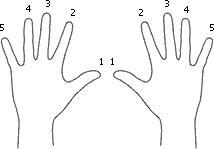
\includegraphics[scale=1]{img/fingers}
    \caption{Kairės ir dešinės rankų pirštų numeracija}
    \label{img:fingers}
\end{figure}

\section{Konvoliucinio tinklo modelis}
\label{appendix:inception_v3}
\begin{figure}[H]
	\centering
	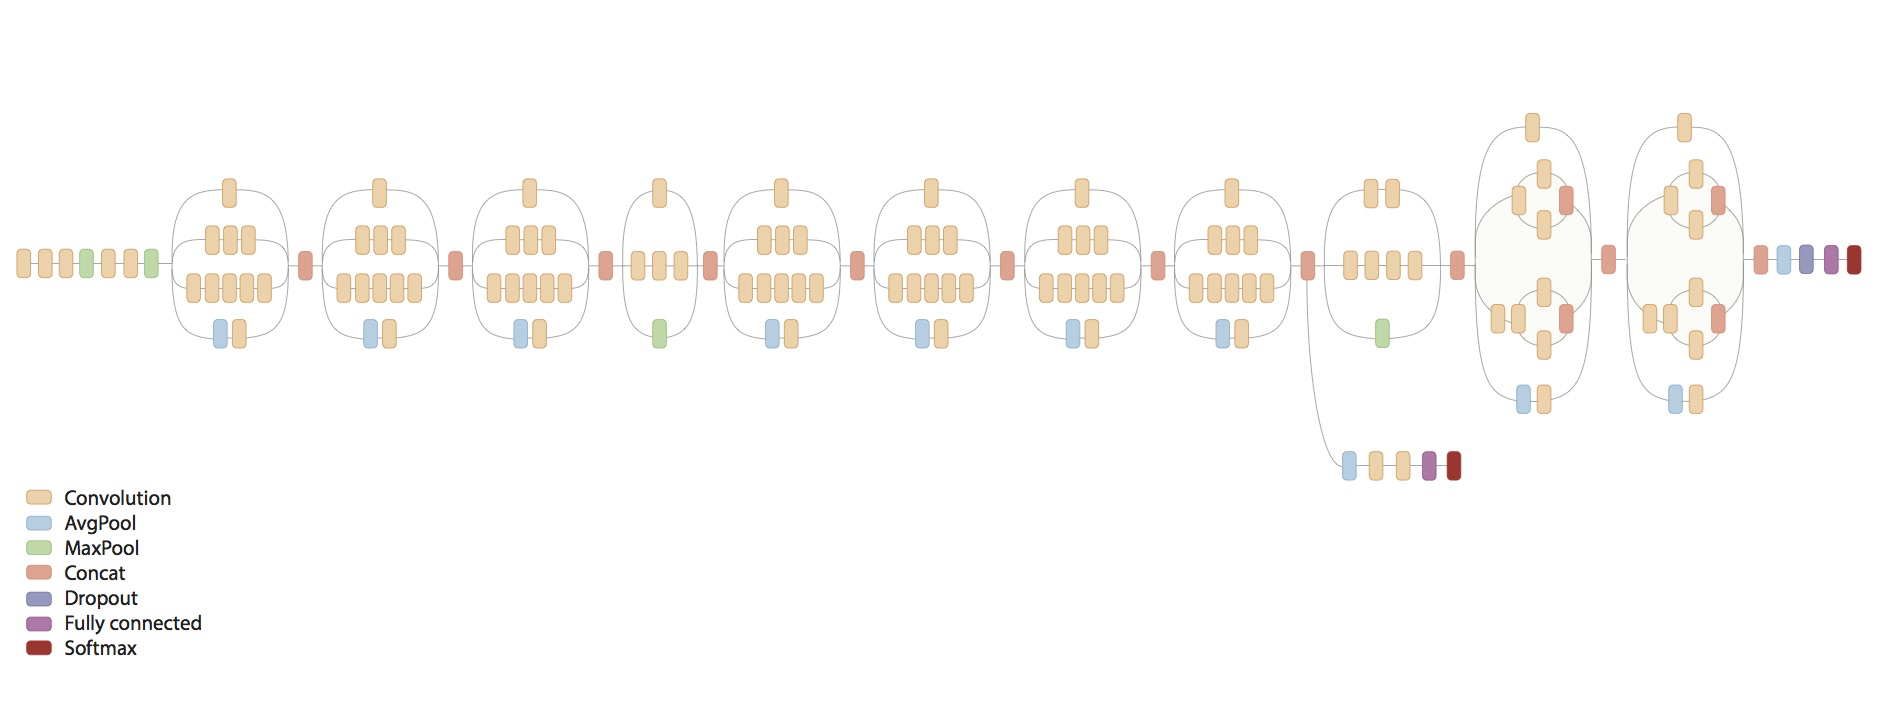
\includegraphics[scale=0.2]{img/inception_v3}
	\caption{Konvoliucinio tinklo modelis „Inception v3“}
	\label{img:inception_v3}
\end{figure}

\section{3 klasių apmokymas}
\label{appendix:3kl}

\textbf{RNT}:
\begin{itemize}
	\item Pirmas bandymas - oranžinė linija
	\item Antras bandymas - mėlyna linija
	\item Trečias bandymas - žydra linija
\end{itemize}

\begin{figure}[H]
	\centering
	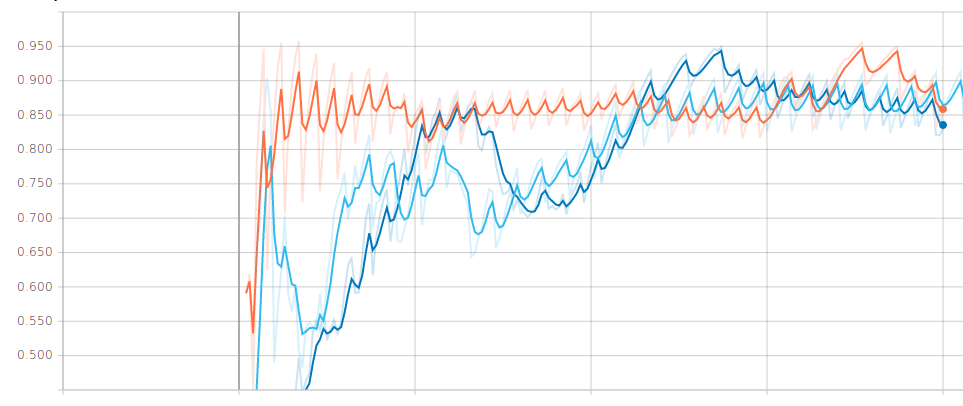
\includegraphics[scale=0.3]{img/1/acc}
	\caption{RNT: Tikslumo grafikas}
	\label{img:3acc}
\end{figure}

\begin{figure}[H]
	\centering
	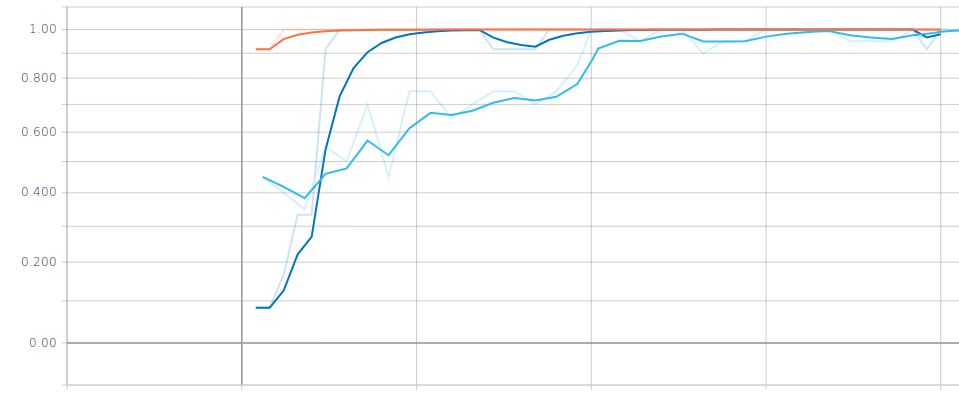
\includegraphics[scale=0.3]{img/1/val}
	\caption{RNT: Pasitikrinimo grafikas}
	\label{img:3val}
\end{figure}

\begin{figure}[H]
	\centering
	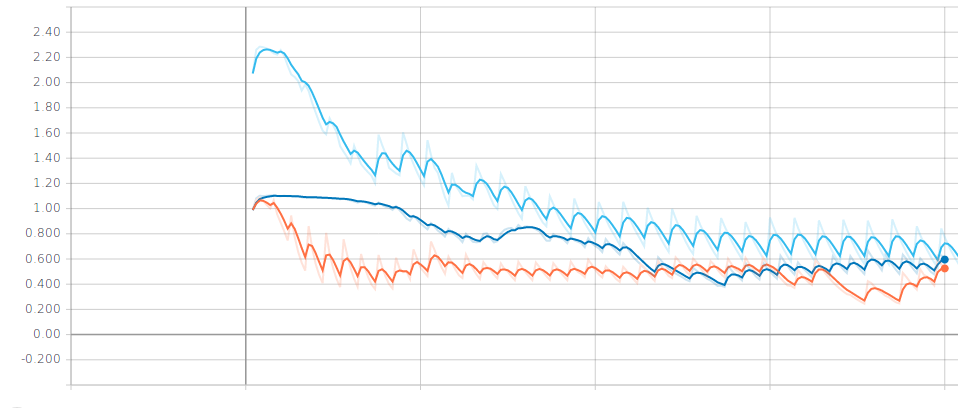
\includegraphics[scale=0.3]{img/1/loss}
	\caption{RNT: Praradimo grafikas}
	\label{img:3loss}
\end{figure}


\section{10 klasių apmokymas}
\label{appendix:10kl}

\textbf{KNT}:
\begin{itemize}
	\item Oranžinė linija - mokymas
	\item Mėlyna linija - pasitikrinimas
\end{itemize}

\begin{figure}[H]
	\centering
	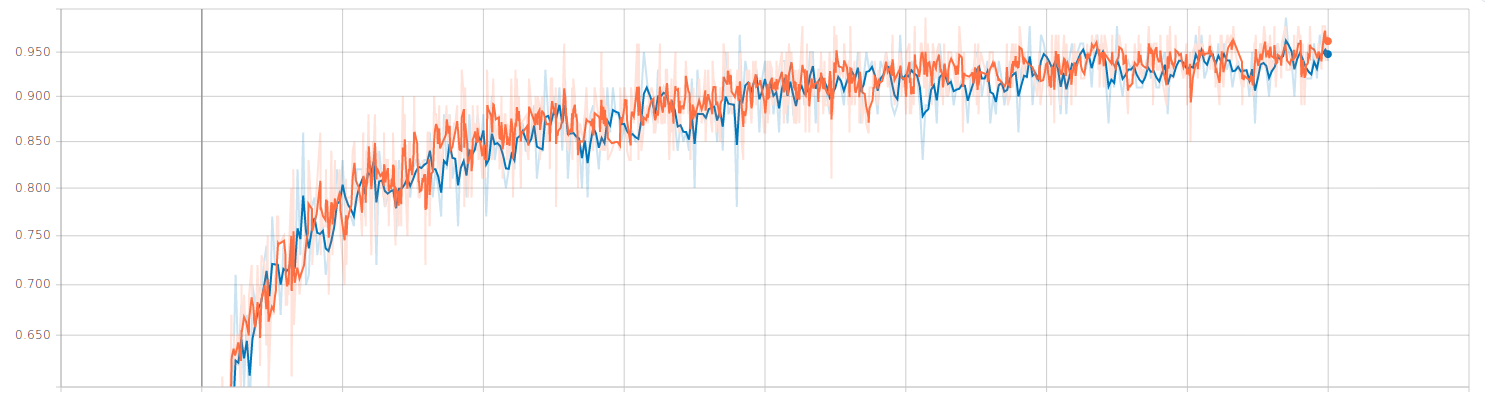
\includegraphics[scale=0.3]{img/2/knn-acc}
	\caption{KNT: Tikslumo grafikas}
	\label{img:10KNT-acc}
\end{figure}


\textbf{RNT}:
\begin{itemize}
	\item Pirmas bandymas - mėlyna linija
	\item Antras bandymas - rausva linija
	\item Trečias bandymas - žalia linija
\end{itemize}

\begin{figure}[H]
	\centering
	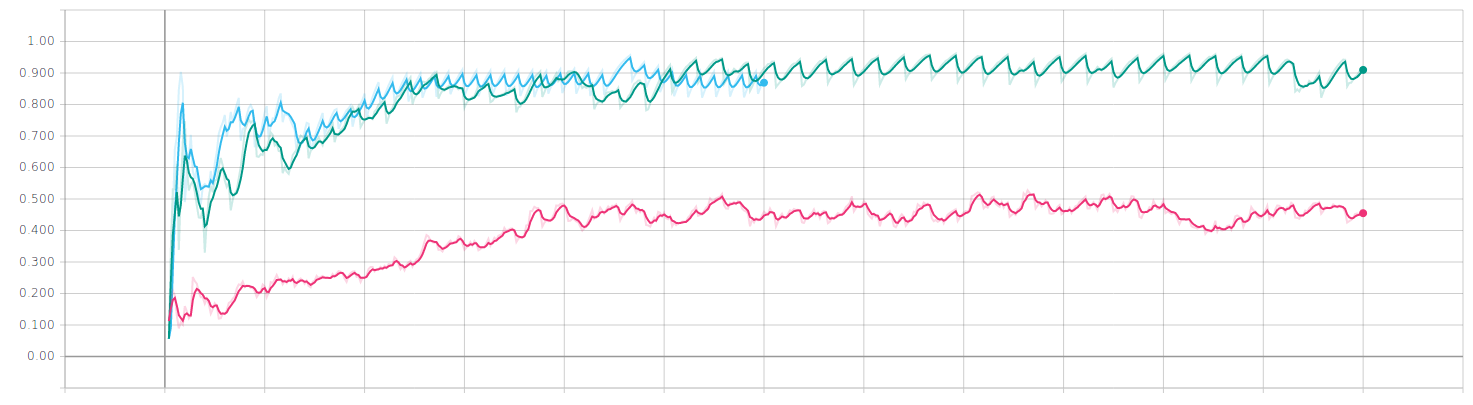
\includegraphics[scale=0.3]{img/2/acc}
	\caption{RNT: Tikslumo grafikas}
	\label{img:10acc}
\end{figure}

\begin{figure}[H]
	\centering
	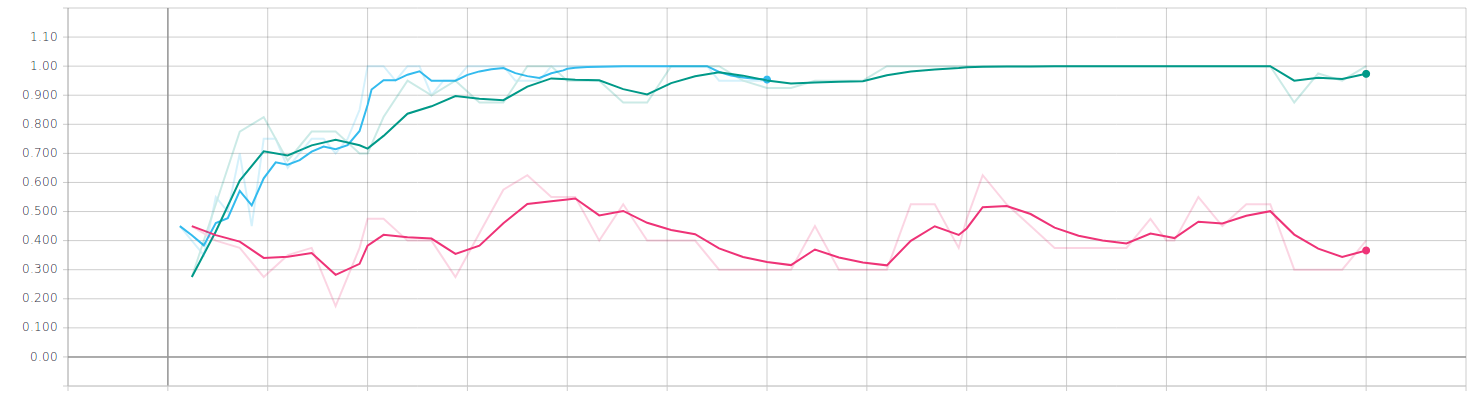
\includegraphics[scale=0.3]{img/2/val}
	\caption{RNT: Pasitikrinimo grafikas}
	\label{img:10val}
\end{figure}

\begin{figure}[H]
	\centering
	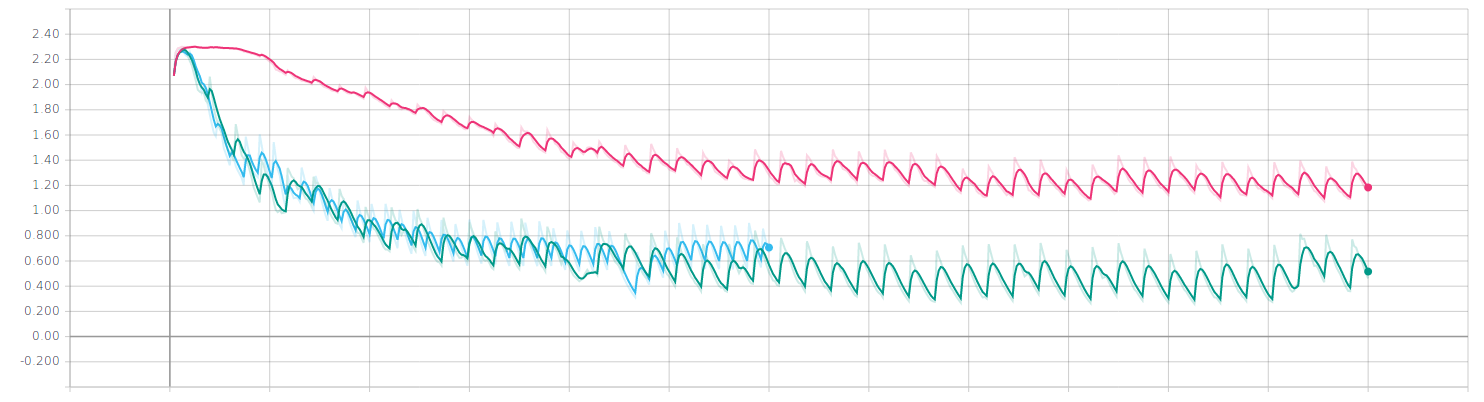
\includegraphics[scale=0.3]{img/2/loss}
	\caption{RNT: Praradimo grafikas}
	\label{img:10loss}
\end{figure}


\section{25 klasių apmokymas}
\label{appendix:25kl}



\textbf{KNT}:
\begin{itemize}
	\item Oranžinė linija - mokymas
	\item Mėlyna linija - pasitikrinimas
\end{itemize}

\begin{figure}[H]
	\centering
	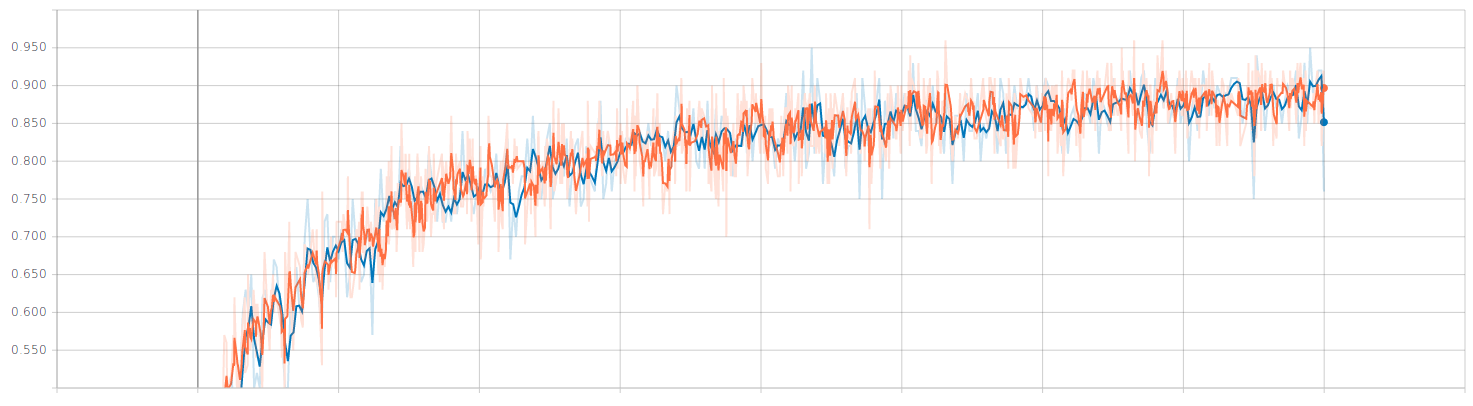
\includegraphics[scale=0.3]{img/3/knn-acc}
	\caption{KNT: Tikslumo grafikas}
	\label{img:25KNT-acc}
\end{figure}

\begin{figure}[H]
	\centering
	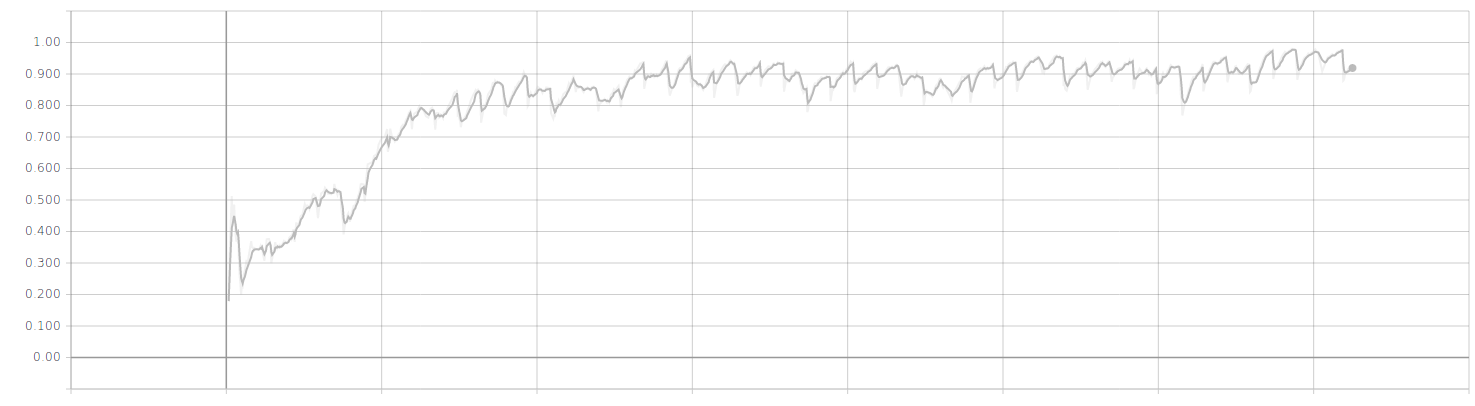
\includegraphics[scale=0.3]{img/3/acc}
	\caption{RNT: Tikslumo grafikas}
	\label{img:25acc}
\end{figure}

\begin{figure}[H]
	\centering
	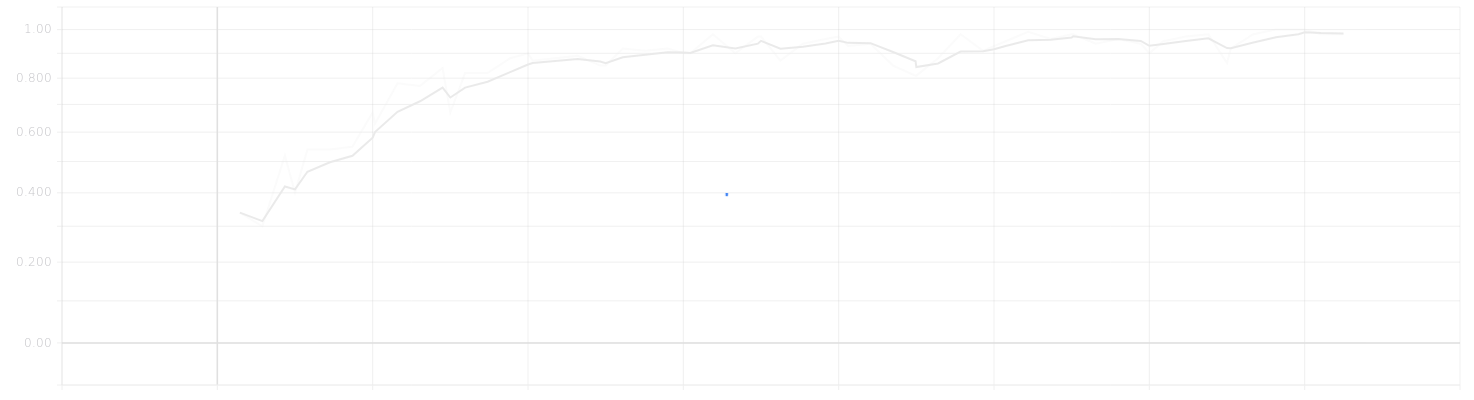
\includegraphics[scale=0.3]{img/3/val}
	\caption{RNT: Pasitikrinimo grafikas}
	\label{img:25val}
\end{figure}

\begin{figure}[H]
	\centering
	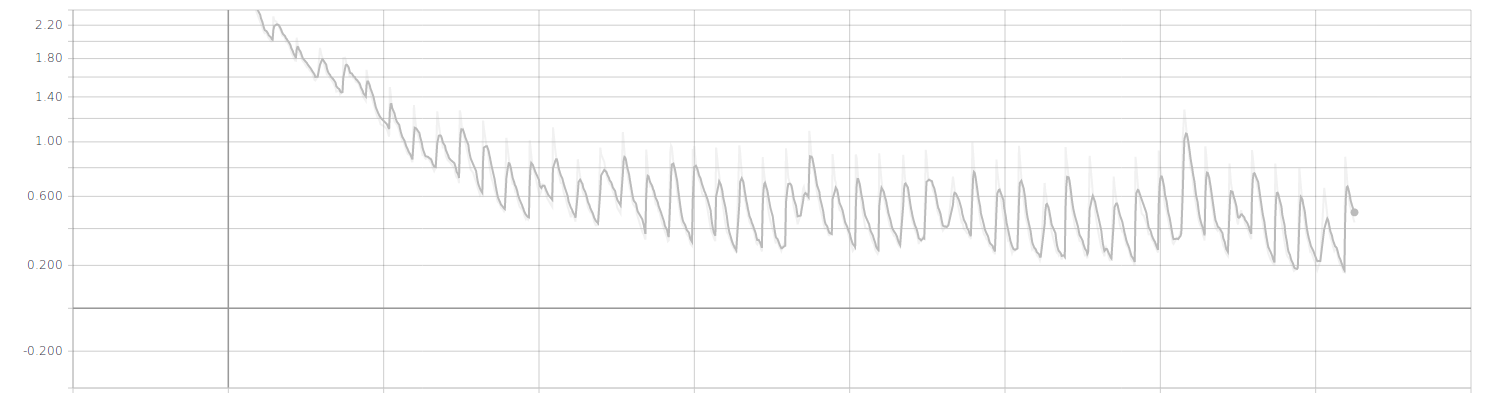
\includegraphics[scale=0.3]{img/3/loss}
	\caption{RNT: Praradimo grafikas}
	\label{img:25loss}
\end{figure}
%\section{Eksperimentinio palyginimo rezultatai}
%% tablesgenerator.com - converts calculators (e.g. excel) tables to LaTeX
%\begin{table}[H]\footnotesize
%  \centering
%  \caption{Lentelės pavyzdys}
%  {\begin{tabular}{|l|c|c|} \hline
%    Algoritmas & $\bar{x}$ & $\sigma^{2}$ \\
%    \hline
%    Algoritmas A  & 1.6335    & 0.5584       \\
%    Algoritmas B  & 1.7395    & 0.5647       \\
%    \hline
%  \end{tabular}}
%  \label{tab:table example}
%\end{table}

\end{document}
